% Journal Article
% LaTeX Template
% Version 1.4 (15/5/16)
%
% This template has been downloaded from:
% http://www.LaTeXTemplates.com
%
% Original author:
% Frits Wenneker (http://www.howtotex.com) with extensive modifications by
% Vel (vel@LaTeXTemplates.com)
%
% License:
% CC BY-NC-SA 3.0 (http://creativecommons.org/licenses/by-nc-sa/3.0/)
%
%%%%%%%%%%%%%%%%%%%%%%%%%%%%%%%%%%%%%%%%%

%----------------------------------------------------------------------------------------
% PACKAGES AND OTHER DOCUMENT CONFIGURATIONS
%----------------------------------------------------------------------------------------

\documentclass[twoside]{article}

 % Package to generate dummy text throughout this template 
\usepackage{multicolrule}
\usepackage{multicol}
\usepackage{graphicx}
\usepackage{subfig}
\usepackage{epigraph}
\usepackage{csquotes}
\usepackage[sc]{mathpazo} % Use the Palatino font
\usepackage[T1]{fontenc} % Use 8-bit encoding that has 256 glyphs
\usepackage{enotez}
\linespread{1.05} % Line spacing - Palatino needs more space between lines
\usepackage{microtype} % Slightly tweak font spacing for aesthetics

\usepackage[spanish]{babel} % Language hyphenation and typographical rules

\usepackage[hmarginratio=1:1,top=32mm,columnsep=20pt]{geometry} % Document margins
%\usepackage[hang, small,labelfont=bf,up,textfont=it,up]{caption} % Custom captions under/above floats in tables or figures
\usepackage{lettrine} % The lettrine is the first enlarged letter at the beginning of the text
\usepackage[all]{nowidow}
\usepackage[backend=bibtex, isbn=false, doi=false]{biblatex-chicago}
\bibliography{final}
\usepackage{url}
\usepackage{enumitem} % Customized lists
\setlist[itemize]{noitemsep} % Make itemize lists more compact


\usepackage{titlesec} % Allows customization of titles
\renewcommand\thesection{\Roman{section}} % Roman numerals for the sections
\renewcommand\thesubsection{\roman{subsection}} % roman numerals for subsections
\titleformat{\section}[block]{\large\scshape\centering}{\thesection.}{1em}{} % Change the look of the section titles
\titleformat{\subsection}[block]{\large}{\thesubsection.}{1em}{} % Change the look of the section titles

\usepackage{fancyhdr} % Headers and footers
\pagestyle{fancy} % All pages have headers and footers
\fancyhead{} % Blank out the default header
\fancyfoot{} % Blank out the default footer
\fancyhead[RE,LO]{\nouppercase{\slshape{\leftmark}}} % Custom header text
\fancyhead[RO,LE]{Mundus Ramonici} % Custom header text
\fancyfoot[RO,LE]{\thepage} % Custom footer text
\fancyfoot[C]{Ramón Serrano Fernández}
\usepackage{afterpage}
\newcommand\myemptypage{
    \null{}
    \thispagestyle{empty}
    \addtocounter{page}{-1}
    \newpage
    }
\usepackage{titling} % Customizing the title section

\usepackage{hyperref} % For hyperlinks in the PDF

%----------------------------------------------------------------------------------------
% TITLE SECTION
%----------------------------------------------------------------------------------------

\setlength{\droptitle}{-4\baselineskip} % Move the title up

\pretitle{\begin{center}\Huge\bfseries} % Article title formatting
\posttitle{\end{center}} % Article title closing formatting
\title{Mundus Ramonici} % Article title
\author{%
\textsc{Ramón Serrano} \\[1ex] % Your name
\normalsize Universidad de Salamanca \\ % Your institution
%\and % Uncomment if 2 authors are required, duplicate these 4 lines if more
%\textsc{Jane Smith}\thanks{Corresponding author} \\[1ex] % Second author's name
%\normalsize University of Utah \\ % Second author's institution
%\normalsize \href{mailto:jane@smith.com}{jane@smith.com} % Second author's email address
}
\date{\today} % Leave empty to omit a date
\renewcommand{\maketitlehookd}{%
}

%----------------------------------------------------------------------------------------

\begin{document}

% Print the title
\newgeometry{left=5cm,right=5cm}
\maketitle
\myemptypage{}
\pagestyle{empty}
\tableofcontents
\restoregeometry{}
\myemptypage{}


\pagestyle{fancy}
\pagenumbering{arabic}

%----------------------------------------------------------------------------------------
% ARTICLE CONTENTS
%----------------------------------------------------------------------------------------

\hypertarget{i-temuxe1tica}{%
  \section{Temática}\label{i-temuxe1tica}}
\epigraph{En un agujero en el suelo, vivía un hobbit.}{\textit{J.R.R Tolkien}\endnote{\autocite*{hobbitprincipio}}}
\begin{multicols}{2}

  \lettrine[nindent=0em,lines=3]{E}l tema principal de este proyecto, si bien creo que ha ido madurando y
  evolucionando a través del propio proceso de creación, y, de algún modo,
  emergiendo y desarrollándose orgánicamente, gira alrededor de la
  fantasía, la creación, y el desarrollo de un mundo personal.

  El enfoque de esta temática central, que he ido manteniendo desde las
  primeras obras, ha sufrido, sin embargo, un cambio drástico: de piezas
  más bien ilustrativas, que comunicaban su intencionalidad apoyándose
  principalmente en el discurso a su alrededor y una simbología críptica,
  han surgido obras, las más tardías, que no se centran tanto en el
  discurso, sino en las metáforas visuales, o incluso en la sensación que
  transmiten. También, el apoyo teórico y la motivación del proyecto ha
  dado un giro importante desde el inicio: al principio, quería crear un
  mundo para crear situaciones con las que comunicar una intencionalidad,
  sobre todo política; pero he descubierto que el mundo ya estaba creado
  en su mayor parte: no ha sido necesario un diseño pormenorizado de
  situaciones ni conceptos extraños, sino más bien una búsqueda de
  sensaciones e imágenes fantásticas, que no surgían de una reflexión
  pragmática sino de una emotiva. Es, por tanto, que considero que aquello
  que quería que fuese un lugar perfectamente definido, se ha tornado en
  algo nebuloso e indeterminado, que sólo toma cohesión y se presenta como
  lugar cuando se observa por partes.

  De la propia reflexión sobre la nebulosa contemplación del mundo ha
  surgido una metareflexión sobre el propio proceso generativo y casi
  errático de la creación de este mundo, y de la naturaleza de la propia
  obra: ¿es esta el mundo creado? ¿o es más bien el proceso agregado de
  creación, con todos los cambios, las ideas incompletas, la evolución de
  las aceptadas y la propia incompletitud e indefinición de muchas partes
  del mismo?

  \begin{center}\rule{0.5\linewidth}{0.5pt}\end{center}

  El por qué de la selección de este tema es ha ido también fluctuando con
  el tiempo, aunque algo menos. Desde muy pequeño me han fascinado todo
  tipo de historias y me considero un ávido lector. También desde pequeño
  he tenido claro que aquello que más me satisfacía era la creación, en el
  sentido amplio de la palabra: las construcciones, dibujar, inventar
  juegos, y, algo más tarde, la robótica, la programáción, la escritura,
  la música o la pintura, han sido algunas de mis aficiones. Aunque no
  tengo muy claro la razón, las historias de fantasía son las que más me
  han fascinado siempre, pasando por el floklore europeo (la mitología
  celta y galesa, la grecorromana, las historias del Rey Arturo, las
  leyendas y romances castellanos), la fantasía juvenil (como las obras de
  Laura Gallego, Brandon Sanderson, Patrick Rothfuss o George R.R.
  Martin), la fantasía mas «académica» o literaria (como puede ser la
  obra de J.R.R Tolkien, Ana María Matute o Neil Gaiman), o los
  videojuegos. De estas historias, lo que más me atrae siempre es la
  existencia de mundos a parte de este, de una manera escapista: la
  curiosidad y la necesidad de explorar lo desconocido y de descubrir que
  no todo es como parece. Esta sensación viene del sentimiento (erróneo),
  de haber perdido la capacidad de asombro ante el mundo, pues está todo
  descubierto.

  Así, en resumidas cuentas, el tema de este proyecto es la
  creación y el descubrimiento orgánicos de un mundo fantástico y propio,
  que emerge de manera automática a partir de un imaginario desarrollado
  pasiva y activamente a lo largo de toda mi vida.

\end{multicols}

\newpage


  \hypertarget{referentes}{%
  \section{Referentes}\label{referentes}}
  \epigraph{It's dangerous to go alone! Take this.}{\textit{The Old Man}\endnote{\autocite*{zelda}}}
  \begin{multicols}{2}
    
    \lettrine[nindent=0em,lines=3]{L}os referentes que he tomado para este proyecto no están escogidos
    \emph{ad hoc} para el proyecto, sino que son los autores y los
    materiales que consumo habitualmente y de los que bebo en la mayoría de
    mis obras, así como en otros aspectos de mi vida.
    
    \hypertarget{literatura}{%
    \subsection{Literatura}\label{literatura}}
    
    En el campo de la literatura, que es en el que más informado y
    experimentado me considero, mis principales fuentes de inspiracion son:
    
  \hypertarget{j.r.r.-tolkien}{%
  \paragraph{J.R.R. Tolkien}\label{j.r.r.-tolkien}}
  
  Tolkien es uno de mis escritores favoritos, y uno de los creadores que
  más admiro. Es indiscutiblemente el padre de la fantasía moderna, y mi
  referente principal en el ámbito más minucioso y quasi-científico de la
  creación de mundos, o \emph{worldbuilding}. De sus obras,
  \emph{El Silmarillion}\autocite*{silmarillion} y \emph{El Señor de los Anillos}\autocite*{esdla} son verdaderos
  tratados y obras cumbres de la creación de un mundo y de cómo infundirle
  vida. \emph{El Hobbit}\autocite*{hobbit} es un cuento que a primera vista parece menor a
  los anteriores, pero considero que es una obra maestra porque alcanza,
  con unas pinceladas muy bien dadas, crear las sensaciones de ese mundo,
  sin la necesidad de pormenorizarlo todo.
  
  \hypertarget{brandon-sanderson}{%
  \paragraph{Brandon Sanderson}\label{brandon-sanderson}}
  
  De los escritores de fantasía en el mercado actual, es mi favorito, y es
  un modelo a seguir en constancia y tesón. Lo que más interesante
  encuentro en este autor, más allá de su maestría con el worldbuilding
  que rivaliza con la de Tolkien, es el énfasis que pone en la creación y
  definición de sistemas de reglas lógicos por los que se rigen sus
  mundos, que les dan una entidad realista a la par que extraña. También
  es muy interesante su \emph{Cosmere} que es el universo en el que se
  desarrollan sus historias, en el que todo está interrelacionado.
  \emph{El Archivo de las Tormentas}\autocite*{sanderson2020} es su obra magna, aunque
  todos sus libros son muy buenos.
  
  \hypertarget{neil-gaiman}{%
  \paragraph{Neil Gaiman}\label{neil-gaiman}}
  
  Neil Gaiman es un escritor que me parece muy interesante, sobre todo por
  la maestría con la que crea sus personajes e imbuye sus mundos de magia
  y misterio sin necesidad de ahondar en detalles. En
  \emph{Stardust}\autocite*{gaiman2021} encontramos referencias a antiguas leyendas británicas,
  así como el concepto de \emph{Otro Mundo} que está tan solo al otro
  lado de una tapia.
  
  \hypertarget{ana-maruxeda-matute}{%
  \paragraph{Ana María Matute}\label{ana-maruxeda-matute}}
  
  De Ana Matía Matute me fascinó \emph{Olvidado Rey Gudú}\autocite*{matute}, en la que el
  mundo se comporta como otro más de los personajes, fluctuante,
  indefinido, y acaba por no haber existido nunca, lo que, en mi opinión,
  le da una capa más de fantasía.
  
  Otros escritores en los que quizá no me inspiro tanto, pero a los que he
  leído y cuyas obras me han influido de alguna otra manera, son por
  ejemplo Andrzej Sapkowski, con su \emph{Saga de Geralt de Rivia}\autocite*{rivia}, Shakespeare,
  sobre todo con obras como \emph{El sueño de una noche de Verano} o
  \emph{Romeo y Julieta}\autocite*{shakespeare}, Gabriel García Márquez, con \emph{Cien años de
  Soledad}\autocite*{garcia} y el Realismo Mágico, William Golding con \emph{La Princesa
  Prometida}\autocite*{goldmanfilipettovidal2013}, o Ursula K. Le Guin, con su saga \emph{Un brujo de
  Terramar}\autocite*{terramar}. También autores más clásicos, como Dante o Bocaccio me
  parecen muy interesantes por su forma de tratar el imaginario legendario
  y místico de la Edad Media.
  
  \hypertarget{artes-pluxe1sticas}{%
  \subsection{Artes Plásticas}\label{artes-pluxe1sticas}}
  
  Dentro de las artes plásticas admiro a casi todos los autores más
  conocidos, aunque si que creo que en este campo no soy tan ducho como en
  el anterior. De algunos autores me interesa mucho su discurso y su
  mensaje, pero también hay muchos otros que me interesan por las técnicas
  que emplean.
  
  \hypertarget{turner}{%
  \paragraph{Turner}\label{turner}}
  
  De Turner me interesa mucho la pseudo abstración y la forma de la que
  emplea el color, anticipándose, en mi opinión, al final del siglo XIX e
  incluso a la Vanguardia. También me atrae mucho la sensación que
  transmite su obra, de frenetismo y desasosiego, sin tener que ahondar en
  detalles a la hora de pintar.
  
  \hypertarget{david-kaspar-friederich}{%
  \paragraph{David Kaspar Friederich}\label{david-kaspar-friederich}}
  
  De Kaspar Friederich, aunque casi toda su obra de paisajes me parece
  magistral, me interesa sobre todo su tratamiento de las ruinas, que
  siempre están ahí para recordar, evocando tiempos pasados y fusionándose
  con la naturaleza.
  
  \hypertarget{el-bosco}{%
    \paragraph{El Bosco}\label{el-bosco}}
    
    De el bosco me fascina la soltura con la que crea situaciones y escenas
    totalmente fantásticas y alocadas, casi surrealistas, además del
    contexto histórico en el que lo hace. También me interesa su uso del
    color, muy profuso y saturado, y, a veces, me parece hasta cómico.
    
    \hypertarget{goya}{%
    \paragraph{Goya}\label{goya}}
    
    De Goya me interesa sobre todo la gestualidad y la forma que tiene de
    crear imágenes con pinceladas muy sueltas, pero que crean el efecto
    correcto a cierta distancia. Sus pinturas negras son una referencia
    importante para algunos obras en tinta.
    
    \begin{center}\rule{0.5\linewidth}{0.5pt}\end{center}
    
    Otros autores que quiero destacar, aunque quizá no hayan sido tan
    influyentes en este proyecto pero que, sin duda, lo son para mi día a
    día, son por ejemplo Leonardo Da Vinci y Durero, de los que me interesa
    la genialidad y el aspecto polifacético del Renacimiento, así como su
    obra más teórica sobre la pintura y sobre los propios materiales
    pictóricos, que es otro tema que me interesa muchísimo. En el campo de
    las técnicas y materiales tradicionales mi fuente antigua de referencia
    es \emph{El Libro del Arte}\autocite{cennini1956}, de Ceninno Ceninni, autor del que se sabe
    poco hoy en día. También cabe destacar en este ámbito a Ralph Mayer,
    aunque su tratado sobre materiales artísticos\autocite*{mayer1948} me parece menos
    interesante por su contemporaneidad. Velázquez, Rubens, Tiziano y
    Tintoretto también están entre mis pintores favoritos, aunque y me
    gustan sobre todo sus obras de mitología. También me interesa mucho
    William Blake, aunque no conozco mucho de su obra.
    
    \hypertarget{muxfasica}{%
    \subsection{Música}\label{muxfasica}}
    
    Dentro de la música, mis referentes principales, como autores, son sobre
    todo Bach y Chopin, pero también me inspiran e interesan mucho la música
    anónima de la Edad Media, las baladas sobre el Rey Arturo, o los
    romances del Romancero Viejo. Ejemplos de estas podrían ser
    \emph{Scarborough Fair}\endnote{\emph{Are you going to Scarborough Fair?\\
    Parsley, sage, rosemary and thyme,\\  Remember me to one who lives there,\\
    For once she was a true love of mine}.\newline Esta es la primera estrofa de la balada,
    que trata de dos enamorados, que habiendo perdido el contacto, se piden favores 
    imposibles
    como prendas de amor. Más información (en inglés) se puede encontrar en este enlace:\\
    https://mainlynorfolk.info/martin.carthy/songs/scarboroughfair.html},o el
    \emph{Romance del Conde Olinos}\endnote{\emph{Madrugaba el Conde Olinos,\\
    mañanita de San Juan,\\
    a dar agua a su caballo\\
    a las orillas del mar}.\newline Este romance es uno de los más conocidos del
    \emph{romancero viejo}, y habla del amor entre la infanta y el conde, que la reina 
    quiere,
    a toda costa, impedir. La letra completa y una interpretación magistral, por Joaquín 
    Díaz, puede encontrarse aquí:\\ https://funjdiaz.net/a_canciones2.php?id=413}. Algunas 
    baladas sobre el mito artúrico, recogidas en el siglo XIX, me han suscitado también 
    mucho interés\endnote{Las baladas se pueden consultar aquí:\\ https://d.lib.rochester.
    edu/camelot/text/six-ballads-about-king-arthur}. Debo destacar también algunas bandas
    sonoras, como la de Howard Shore para \emph{El Señor de los Anillos}, o
    la de Koji Kondo para \emph{The Legend of Zelda}, que, aunque son
    acompañamiento a obras que ya he mencionado, han jugado un papel muy
    importante para mí.
    
    \hypertarget{videojuegos}{%
    \subsection{Videojuegos}\label{videojuegos}}
    
    Los videojuegos han sido una parte muy importante de mi vida desde la
    infancia, y creo no equivocarme al afirmar que muchos de ellos se pueden
    considerar arte sin lugar a dudas.
    
    \hypertarget{the-legend-of-zelda}{%
    \paragraph{The Legend of Zelda}\label{the-legend-of-zelda}}
    
    Es mi saga de videojuegos favorita, y posiblemente una de las
    influencias más grandes de este proyecto. Dentro de los más de veinte
    títulos que la componen, destacaría \emph{Skyward Sword}\autocite*{miyamoto} y \emph{Breath
    of The Wild}\autocite*{miyamoto2}, sobre todo por la sensación de explorar lo desconocido 
    que
    transmiten, de adentrarse en un mundo extraño que nunca antes has visto.
    También es muy interesante \emph{Majora's Mask}\autocite*{miyamoto3} por el mundo hostil y
    desconocido que presenta, como un reflejo oscuro de Hyrule.
    
    \hypertarget{minecraft}{%
    \paragraph{Minecraft}\label{minecraft}}
    
    Creo que \emph{Minecraft}\autocite*{persson} es otro de los juegos que más me ha influido,
    sobre todo por la libertad que otorga al jugador de hacer con el mundo
    que se le presenta aquello que le plazca.
    
    \begin{center}\rule{0.5\linewidth}{0.5pt}\end{center}
    
    Otros videojuegos que me parecen interesantes y que me han influido,
    aunque en menor medida, son, por ejemplo, \emph{Skyrim},
    \emph{Civilization}\autocite*{meier}, \emph{Final Fantasy IX} o \emph{The Witcher}.
    
    \hypertarget{informuxe1tica}{%
    \subsection{Informática}\label{informuxe1tica}}
    
    En contraposición al enorme interés que me causa el estudio de la evolucón histórica de 
    los materiales y técnicas artísticas, y la búsqueda en mi obra de una vuelta a esas 
    recetas artesanas y casi de alquimia de principios del renacimiento como las que expone 
    Cennini, desde pequeño he desarrollado una enorme curiosidad por la tecnologia y un deseo 
    de dominarla. En esto influye indudablemente mi entorno: desde la infancia me he visto 
    rodeado, si no de la última tecnología, de mis padres, programadores ambos, y que, sobre 
    todo a principios de siglo fueron pioneros de la informática, los negocios on-line, el 
    hardware, y el software.
    
    Creo que, de hecho, fue en el diseño web como se empezó a gestar mi interés por el diseño, 
    la estética y la composición, hecho que, juto con varios otros, me ha traído a donde 
    estoy. Desde entonces, mis intereses en el campo tecnológico e informático han tendido 
    sobre todo a los campos más teóricos, como la arquitectura de sistemas, la implementación 
    de lenguajes de programación o la propia historia de la informática.
    
    En este proyecto he intentado aunar mi pasión e interés por la informática junto con mi 
    visión artística y la creación de mundos, y, aunque al final, más que de manera práctica 
    lo he hecho de manera referencial, en mi investigación he encontrado recursos y ramas en 
    las que estas dos disciplinas --- arte y programación, la \emph{programación creativa}, 
    que dispone de recursos como \emph{Nannou}\autocite*{nannou}, un software que permite 
    programar una amplia gama de demostraciones visuales, auditivas o incluso con láseres, o 
    \emph{Processing}\autocite*{processing}, un entorno que pretende facilitar la programación 
    de este tipo de aplicaciones--- se entrelazan de manera muy interesante. También he 
    encontrado inspiración en la cultura \emph{maker}, de la que se puede decir que formo 
    parte más o menos activa, en la que se dan iniciativas como \emph{Arduino}\autocite*
    {arduino} o \emph{Raspberry Pi}\autocite*{raspberry}, en la \emph{demoscene}\autocite*
    {demoscene}. Recursos y referentes en estos campos son, por ejemplo, la revista \emph
    {Hackaday}\autocite*{hackaday}, el libro \emph{The Nature Of Code}\autocite*{shiffman2012}
    , o, en un ámbito puramente teórico, el canal de \emph{Youtube Computerphile}\endnote{El 
    canal \emph{Computerphile} se puede encontrar en este enlace:\\ https://www.youtube.com/
    user/Computerphile}, de la Universidad de Nottingham, en el que participan regularmente 
    figuras de gran calado como Brian Kernighan, desarrollador del lenguaje \emph{C}\autocite*
  {cprogramming}, o el Profesor Brailsford, uno de los miembros del comité encargado del 
  diseño del formato \emph{PDF}.
  
  Otras influencias y referencias, importantes pero más generales son por
  ejemplo todas las leyendas del folklore gaélico (galesas, irlandesas y
  escocesas, así como gallegas y bretonas), sobre el Mundo de las Hadas ---
  \emph{Ávalon}, \emph{Anwwn} o \emph{Tír na nÓg}---, el concepto romano
  equivalente de \emph{Orbis Alia}, y la mitología relacionada con este
  mundo, así como sus personajes recurrentes: \emph{Arawn} u
  \emph{Oberón}, y \emph{Titania}, rey y reina de las hadas y del más allá, \emph{Taliesin}, 
  el bardo quasi legendario al que a veces se asocia con \emph{Myrddin Wyllt o Emrys}, que 
  es el precedente del Merlín artúrico y del estereotipo de sabio y mago de la cultura 
  popular. También me interesan mucho las mitologías góticas y neo-góticas y de fantasía 
  urbana como las
  historias de vampiros --- tanto las clásicas como \emph{Drácula}\autocite*{stoker}, o 
  contemporáneas como \emph{Entrevista con el Vampiro}\autocite*{rice1994} o el \emph{Mundo 
  de Tinieblas}\autocite*{achilli2016}.
  
\end{multicols}

\newpage
\hypertarget{enfoque}{%
  \section{Enfoque y Marco Teórico}\label{enfoque}}
\epigraph{Vida antes que muerte\\Fuerza antes que debilidad\\Viaje antes que destino}{\textit{Kaladin Benditormenta}\endnote{\autocite*{sandersonjuramento}}}
\begin{multicols}{2}

  \lettrine[nindent=0em,lines=3]{E}l enfoque del proyecto es lo que más ha cambiado desde su concepción
  hasta el momento final. En un principio, la intecnción era criticar
  ciertas conductas y situaciones que se dan en nuestro contexto actual a
  través de la presentación del mundo como una suerte de parábola. Uno de
  los temas que más me interesaba era el de la juventud, la preocupación
  por el legado que nos dejarán las generaciones que ahora están a cargo
  de todo, y la reivindicación de nuestra identidad propia y nuestros
  derechos como personas con la misma legitimidad que gente más mayor. A
  medida que el proyecto ha ido evolucionando me he dado cuenta de que lo
  que en realidad he hecho ha sido hablar de mí: de mis sueños, mis
  ideales, del mundo que me gustaría, de mi propia evolución personal y de
  cómo se hha desarrollado mi imaginario personal desde la niñez hasta el
  momento presente. Es un proyecto ciertamente intimista, que trata un
  tema muy ligado con todos los aspectos de mi vida como lo es el afán y
  la necesidad de crear, pero no para hacer reivindicaciones ni para
  mostrarlo, sino porque lo hago de forma natural. En realidad, siento que
  una de las reflexiones más importantes que he obtenido es la de que,
  para mí y sobre mi trabajo, es mucho más importante, satisfactorio, e
  incluso llegaría a decir que, donde reside la materia artística, es en
  el proceso, en la creación, que sucede en el momento en el que se
  proyecta, se piensa o se tiene una idea. Aunque considero importantes la
  materialización y el desarrollo de esas ideas, pues muchas veces surgen
  a partir de ellas otras nuevas, creo poder afirmar que la obra y lo
  artístico, al menos en mi trabajo, está en la idea virtual, en el
  pensamiento, intangible y nebuloso, y el lienzo o la realización de la
  misma no es más que una manera de recordarla, comunicarla, y
  registrarla.

  Sobre la teoría involucrada en este proyecto, quiero hacer una
  distinción clara entre dos conceptos que se desarrollan paralelamente en
  el mismo, cuyos discursos teóricos difieren ampliamente en naturaleza.
  El primero, la teoría, técnica y estrategias empleadas para la creación
  de mundos, es relativamente sistemático y utilitarista, y trata, sobre
  todo, de cómo se crean mundos fantásticos efectivos, apoyándose en los
  propios métodos que usan escritores de renombre y en el consenso de la
  comunidad especializada en torno a ello, y de cómo esto que proviene del
  ámbito literario se puede adaptar al pictórico y plástico en general. El
  segundo es el discurso que emana de mi propio proceso creativo, de mi
  visión conjunta del mundo ficticio, más reflexivo y centrado en cómo se
  percibe la creación del mundo como obra.

  \hypertarget{de-la-creaciuxf3n-de-mundos}{%
    \subsection{De la Creación de
      Mundos}\label{de-la-creaciuxf3n-de-mundos}}

  En el ámbito literario, específicamente en el de la literatura
  fantástica y juvenil de los últimos años, ha surgido la tendencia de
  seguir ciertas reglas, métodos y estrategias más o menos definidas, así
  como diversos acercamientos, para conseguir envolver las obras en un
  buen \emph{worldbuilding}, esto es, creación de mundos. Diversas
  comunidades de \emph{worldbuilders}\autocite*{worldbuilding} se esparcen por internet y 
  son realmente interesantes y accesibles a través de \emph{Reddit}, existiendo incluso 
  algunas subcomunidades muy específicas como la de quienes se dedican a diseñar lenguas 
  artificiales o \emph{conlangs}\autocite*{conlangs}. Algunos de las estrategias más 
  utilizadas por estas comuidades son, por ejemplo, la definición exhaustiva de unos 
  sistemas físicos y cosmológicos en base a los reales, y, a través del análisis de los 
  mismos y la comparación, intentar deducir los resultados del mundo a nivel general (clima, 
  orografía, vegetación, biología), e ir diseñando incrementalmente unas sociedades que se 
  adaptan a estos sistemas. Otras técnicas más sencillas pueden ser la creación incremental 
  del munco a partiir de una idea base, la definición de conceptos de mayor a menor 
  generalidad o viceversa, o tomar como punto de partida ucronías, distopías o utopías.

  Cabe destacar además de estas técnicas, que existen recursos que proceden de fuentes 
  extremadamente valoradas en el campo, como pueden ser las \emph{Cartas de Tolkien}
  \autocite*{cartast}, un compendio de la correspondencia que llevó Tolkien a través de su 
  vida, íntimamente relacionadas con la \emph{Tierra Media}, o \emph{Historia de la Tierra 
  Media}\autocite*{historiamedia}, una verdadera enciclopedia y registro del proceso 
  creativo de Tolkien a través de toda su vida, ambos publicados y recopilados póstumamente 
  por su hijo, Christopher Tolkien. Más contemporáneas y centradas en una creación de mundos 
  más rápida y efectista son las clases magistrales de Brandon Sanderson en la Universidad 
  Joven de Brigham, disponibles en su canal de \emph{YouTube}\endnote{El canal de \emph
  {YouTube} de Brandon Sanderson se encuentra en el siguiente enlace:\\ https://www.youtube.
  com/user/BrandSanderson} (de las que publicará un libro dentro de poco tiempo), además de 
  su propia página personal, donde escribe artículos y detalla su proceso de 
  escritura\autocite*{sanderson2020}.

  En cuanto a cómo se pueden aplicar algunos de estos métodos a la pintura
  y a la plástica, queriendo que estas sean la obra principal, creo que es
  sencillo si abstraemos la parte de creación del proceso y nos centramos
  en la parte de realización y de cómo se enseña el mundo. Uno de los
  preceptos casi unánimemente aceptados por los \emph{worldbuiders} es el
  de evitar el exceso de información que se da al espectador (lector en el
  caso literario) de golpe, sobre el mundo (conocido como
  \emph{infodumping}), y esto es aplicable, incluso más, a la pintura: la
  forma más efectiva de dar a conocer el mundo creado es conseguir
  transmitir \emph{las sensaciones que en él se experimentan}, crear una
  atmósfera única y distintiva, en lugar de llenar la obra de referencias
  y simbolismos crípticos que necesitan de una explicación compleja y un
  contexto extenso sobre el mundo.

  \hypertarget{del-proceso-de-creaciuxf3n}{%
    \subsection{Del proceso de
      creación}\label{del-proceso-de-creaciuxf3n}}

  Una reflexión muy interesante que surge del proceso de la propia
  creación del mundo y a la que ya he hecho referencia es la de cómo se
  desarrolla y cómo se visualiza de una manera general y homogénea el
  mundo, desde la visión del autor, que lo contempla todo como un
  conjunto. Esto me ha llevado a desgranar una cierta sistemática y
  cosmovisión alrededor del mundo, en constante cambio, que define las
  bases que lo componen y su razón de ser, todo ello en relación a la
  disposición del proyecto a medida que crecía, sobre una de las paredes
  del taller.

  Esta pared, que es, más allá que el espacio físico, la idea en conjunto
  del proyecto, es el proceso de creación, y a la vez la muestra y ventana
  del mundo creciente. Este mundo se da a conocer a través de ciertas
  \emph{reglas sistemáticas}, \emph{imágenes sinestésicas}, sin procesar,
  e \emph{ideas}, en diversos grados de maduración e importancia, tanto
  visuales como escritas y abocetadas. Las reglas le dan \emph{coherencia}
  al mundo, permitiendo, con una definición simple, la derivación sin
  necesidad de intervención por parte del autor, una evolución orgánica.
  Las imágenes sinestésicas le dan \emph{sensibiliad} y \emph{presencia},
  una suerte de alma, que no es ni cómo se comporta, ni cómo es, sino
  \emph{cómo se siente}. Las ideas le dan \emph{intención}, y
  \emph{entidad}: más allá de su evolución elemental y las reglas por las
  que se rige, que pueden ser incluso ignoradas por alguien profano sin
  restarle valor al mundo, o cómo se sienten sus realidades y su
  \emph{atmósfera}, son su carácter, cómo \emph{es} y cómo \emph{existe}.

  Estas paredes o mapas mentales, son, por tanto, una instantánea agregada
  de todo este conjunto, en el que todo se pliega y se solapa en torno al
  concepto abstracto que el autor tiene en mente cuando piensa en su
  creación.

\end{multicols}

\newpage
\hypertarget{planteamiento-metodoluxf3gico}{%
  \section{Planteamiento
    Metodológico y Técnico}\label{planteamiento-metodoluxf3gico}}
\epigraph{El fundamento del arte (...) requiere lo siguiente: saber trituar, moler, encolar, aparejar, enyesar, (...) dorar, bruñir, templar...}{\textit{Ceninno Ceninni}\endnote{\autocite*{arteiv}}}
\begin{multicols}{2}

  \lettrine[nindent=0em,lines=3]{A}poyándome en las bases teóricas anteriormente expuetas, tanto las
  propias como las adaptadas de la literatura, a lo largo del proyecto me
  he ido centrando, sobre todo, en crear \emph{imágenes sinestésicas} e
  \emph{ideas}. Aunque ha habido intentos de crear y desarrollar algunas
  \emph{reglas sisetemáticas}, no he hallado una forma elegante de
  incluirlas como obras por derecho propio y aisladas, sino que arropan y
  dan contexto como bocetos, apuntes, y pruebas de concepto, superpuestas
  y llenando los huecos entre obras e ideas de otra índole alrededor de
  \emph{la pared} --- en verdad, ¿por qué no considerarlas como obras por
  derecho propio, aunque expresadas de manera diferente? A lo que me
  quiero referir es que no he conseguido o necesitado conferirles una
  materialidad pictórica. De una u otra manera, creo que al quedar cada
  obra confinada a un tipo de estos «bloques básicos» del mundo, el
  resultado es un trabajo limpio, que se puede sostener por si mismo, pero
  que de igual manera gana profundidad al rodearlo de los elementos de
  \emph{la pared}.

  Formalmente, y más que a partir de una decisión meditada, através de la
  experimentación y la creación iterativa, he dado en formalizar como
  paisajes «pseudo-abstractos» (esto es, que, sin tener una idea en mente
  sobre lo que iba a pintar, los resultados se pueden interpretar como
  paisajes) y algunas otras imágenes muy sueltas las \emph{imágenes
    sinestésicas}, y como arquitecturas, algunos retratos y paisajes más
  figurativos las \emph{ideas}. Esto se amolda razonablemente bien a la
  propia definición de estos conceptos, pues a través de las
  \emph{imágenes sinestésicas} pretendo transmitir sensaciones y una
  atmósfera, y, através de las \emph{ideas}, la materialidad y realidad
  del mundo.

  La metodología de trabajo empleada para desarrollar el proyecto ha ido
  cambiando a medida se producían los cambios en torno a temática, enfoque
  e intencionalidad ya mencionados.

  En los primeros trabajos, las ideass surgían más lentamente, y la
  mayoría de las veces, sin reflexionar mucho, y tendía a no barajar más
  ideas que la primera (centrando algunas veces demasiado esfuerzo para
  hacerla encajar, aunque fuese forzosamente). A medida que progresaba, he
  ido desarrollando una metodología de trabajo más sosegada, y, aunque no
  muy centrada en la reflexión teórica o en la investigación, que han
  surgido eminentemente \emph{a posteriori}, sí en la introspección y el
  la observación de mi obra previa. Aunque, sin duda, muy guiado por la
  intuición, defino este proceso como más sosegado porque se caracteriza
  por la importacia de los bosquejos y bocetos previos al planteamiento de
  la obra, que actúan como documento de reflexión tanto teórica como
  plástica: en todos los proyectos, la idea evoluciona fundamentalmente
  sobre el papel (o el propio código o el lenguaje), unos primeros esbozos
  muy rápidos, bocetos de detalle y gradualmente más encauzados, hasta
  llegar a pruebas de color y bocetos finales de línea.

  \hypertarget{estrategias-conceptuales}{%
    \subsection{Estrategias conceptuales}\label{estrategias-conceptuales}}

  Las estrategias conceptuales a las que más partido les he sacado en este
  proyecto han sido sobre todo los recursos de la retórica visual, como
  metáforas y analogías, las indefiniciones --- dejar que el espectador
  interprete las partes de la imagen y reconstruya la escena en base a su
  percepción subjetiva, si bien no referido a la abstracción o la
  interpretación de los conceptos, sí a la de los espacios, como las
  perspectivas, o las direcciones.

  \hypertarget{estrategias-pluxe1sticas}{%
    \subsection{Estrategias plásticas}\label{estrategias-pluxe1sticas}}

  Las estrategias plásticas que he ido empleando a través del proyecto han
  sido fruto en su mayoría de un proceso de experimentación con el
  material. La técnica que más he usado a lo largo del proyecto ha sido el
  óleo: los efectos más interesantes que han surgido con este han sido las
  texturas casi de acuarela que he conseguido con la superposición de
  manchas muy diluidas y difuminadas. El temple es otra técnica con la que
  he experimentado, aunque algo menos. Los usos más interesantes de este
  me han resultado al mezclar el pigmento con muy poca yema, creando unas
  texturas muy terrosas, casi de tiza, de colores muy vivos.

  En cuanto al uso del color, a medida que el proyecto avanzaba, se hacía
  más protagonista la gama cromática completa, muy superpuesta, y muchas
  veces casi sin mezclar, creando así unas superficies irreales y
  fantásticas como las que buscaba. También cabe destacar la importancia
  de la gestualidad en algunas obras, casi abstractas, la incompletitud
  deliberada de algunas partes, que deja patente el proceso, y el uso de
  imprimaciones y materiales caseros.
\end{multicols}
\newpage

\hypertarget{conclusiones}{
  \section{Conclusiones}\label{conclusiones}}
\epigraph{Te considero una gran persona, señor Bolsón, y te aprecio mucho; pero en última instancia ¡eres sólo un simple individuo en un mundo enorme!}{\textit{Gandalf el Gris}\endnote{\autocite*{gandalf}}}
\begin{multicols}{2}

  \lettrine[nindent=0em,lines=3]{O}bservando el recorrido del proyecto, creo que tengo claro qué tipo de
  obra y procedimientos funcionan bien: la simplicidad en la
  representación es clave para crear obras rápidas y efectivas, y creo que
  es la manera idónea para transmitir el cambio constante del mundo que
  pretendo crear. Queda también patente que presentar este tipo de obra
  como un conjunto, rodeada de bocetos, ideas, proyectos nacientes, todo
  ello en un espacio que evoluciona, es un acierto y una propuesta
  expositiva interesante.

  La investigación y el tiempo invertido en este proyecto, ha dado sus
  frutos, aunque ha habido momentos de frustración y de sequía de ideas.
  Sobre todo ha sido un proceso de introspección muy interesante, que ha
  suscitado reflexiones realmente importantes, ya no solo sobre el propio
  proyecto, sino sobre mi proceso creativo, mi visión del arte, mis
  motivaciones y mis intenciones, y creo que esto es realmente valioso.

  La creación de este mundo es algo que no se acota solamente al presente
  proyecto, sino que es algo que viene de lejos y que continuará iterando,
  sobreescribiéndose y cambiando, difuso, durante mucho tiempo más.
  También ha sido muy satisfactoria la creación de algunas de las obras
  que lo componen, y la sensación de completitud al ir atando cabos entre
  diferentes conceptos, y de conseguir hilar el propio discurso de una
  manera coherente y clara.

  En el periplo de búsqueda de inspiración para nuevos tipos de obra y de
  representar el mundo, también me he topado con un tema muy interesante y
  que llevaba buscando mucho tiempo: la solución al problema que se me
  había planteado al intentar unir mi interés por la informática y la
  programación, y las artes, la «programación creativa», o \emph{creative
    coding}. Esta es una rama muy interesante tanto de la ingeniería
  informática, como de las artes digitales y gráficas, que pretende crear
  arte interactivo de manera procedural, matemática y programática.

  En conclusión, este proyecto me deja con buen sabor de boca, y con la
  seguridad de haber desarrollado un estilo y un lenguaje propios
  relativamente maduro, así como el descubrimiento de nuevos campos para
  explorar.
\end{multicols}
\newpage

\hypertarget{anexo-exposiciuxf3n-del-proyecto}{%
  \section{Anexo: Exposición del
    proyecto}\label{anexo-exposiciuxf3n-del-proyecto}}
\begin{multicols}{2}

  \lettrine[nindent=0em,lines=3]{E}ste proyecto se expone como un diálogo entre las dos facetas ya mencionadas:
  el ámbito más plástico y tradicional de la pintura, y el campo de lo virtual,
  programático e informático. No pretendo distinguir las dos vertientes como
  mutuamente exclusivs, sino complementarias. Así lo he querido dar a entender
  a través de la inclusión de elementos de una en otra (los bocetos en la virtual,
  listados del código fuente en la física). Así como todo el material, referencias y
  obras empleadas está incluido en este anexo, todo el que atañe a la esencia técnica
  de la exposición virtual (y el proceso de su creación y evolución), junto con el código
  fuente para el último, así como una copia de este documento y las licencias pertinentes
  se encuentran alojados en el siguiente repositorio de \emph{GitHub}\endnote{Enlace al repositorio del proyecto: https://github.com/uri-nyx/ProyectoFinal}, en el que se adjuntan
  instrucciones para su correcta instalación y experimentación.

  Este formato intenta emular el espacio expositivo ideal en el que se
  expondría este proyecto, además de aprovechar las capacidades del medio
  para disponer multiplicar, redimensionar y contravenir las leyes
  naturales en pos de conseguir crear un espacio irreal que asemeje a la
  idea, difusa y abstracta, que existe del mundo construido en la mente
  del autor.
\end{multicols}
\hypertarget{relaciuxf3n-de-obras}{%
  \subsection{Relación de obras}\label{relaciuxf3n-de-obras}}
  Las obras, que se presentan a continuación, listadas por orden de aparición, son aquellas de la
  pared que considero, por uno u otro motivo (estética, apego emocional o significancia ccon respecto
  a los temas tratados), como las principales de \emph{la pared}. Adjuntos a este documento y en el
  ya enlazado repositorio se pueden encontrar obras que considero menos importantes, así como bocetos,
  apuntes, reflexiones y pruebas de todo tipo. También cabe destacar que algunas de las obras que aquí
  se listan fueron en principio bocetos y esbozos de los que partieron otras. Sin embargo, creo que su
  valor, tanto estético como documentas (al ser un registro primario del proceso creativo), bien valen 
  su inclusión en esta relación.

  \begin{enumerate}
    \item \textit{Camino entre los bosques}: temple sobre cartón, 20x75cm.
    \item \textit{Camino entre las nubes}: temple sobre tabla, 20x80cm.
    \item \textit{El ojo del Dragón}: óleo sobre cartón, 20x75cm.
    \item \textit{Oberón cruzando las puertas de Ávalon}: oleo sobre papel, 50x70cm.
    \item \textit{Las puertas de Even}: óleo sobre sábana, 60x75cm.
    \item \textit{Diseño de las puertas de Even}: tinta sobre papel, 35x50cm.
    \item \textit{El faro}: acuarela sobre papel, A4.
    \item \textit{Un mar de nubes}: acuarela sobre papel, 30x20cm.
    \item \textit{El invierno}: temple y óleo sobre tabla, 60x75cm.
    \item \textit{La Sofi}: tinta ferrogálica sobre papel, A3.
    
  \end{enumerate}

  \newpage
  \begin{center}
    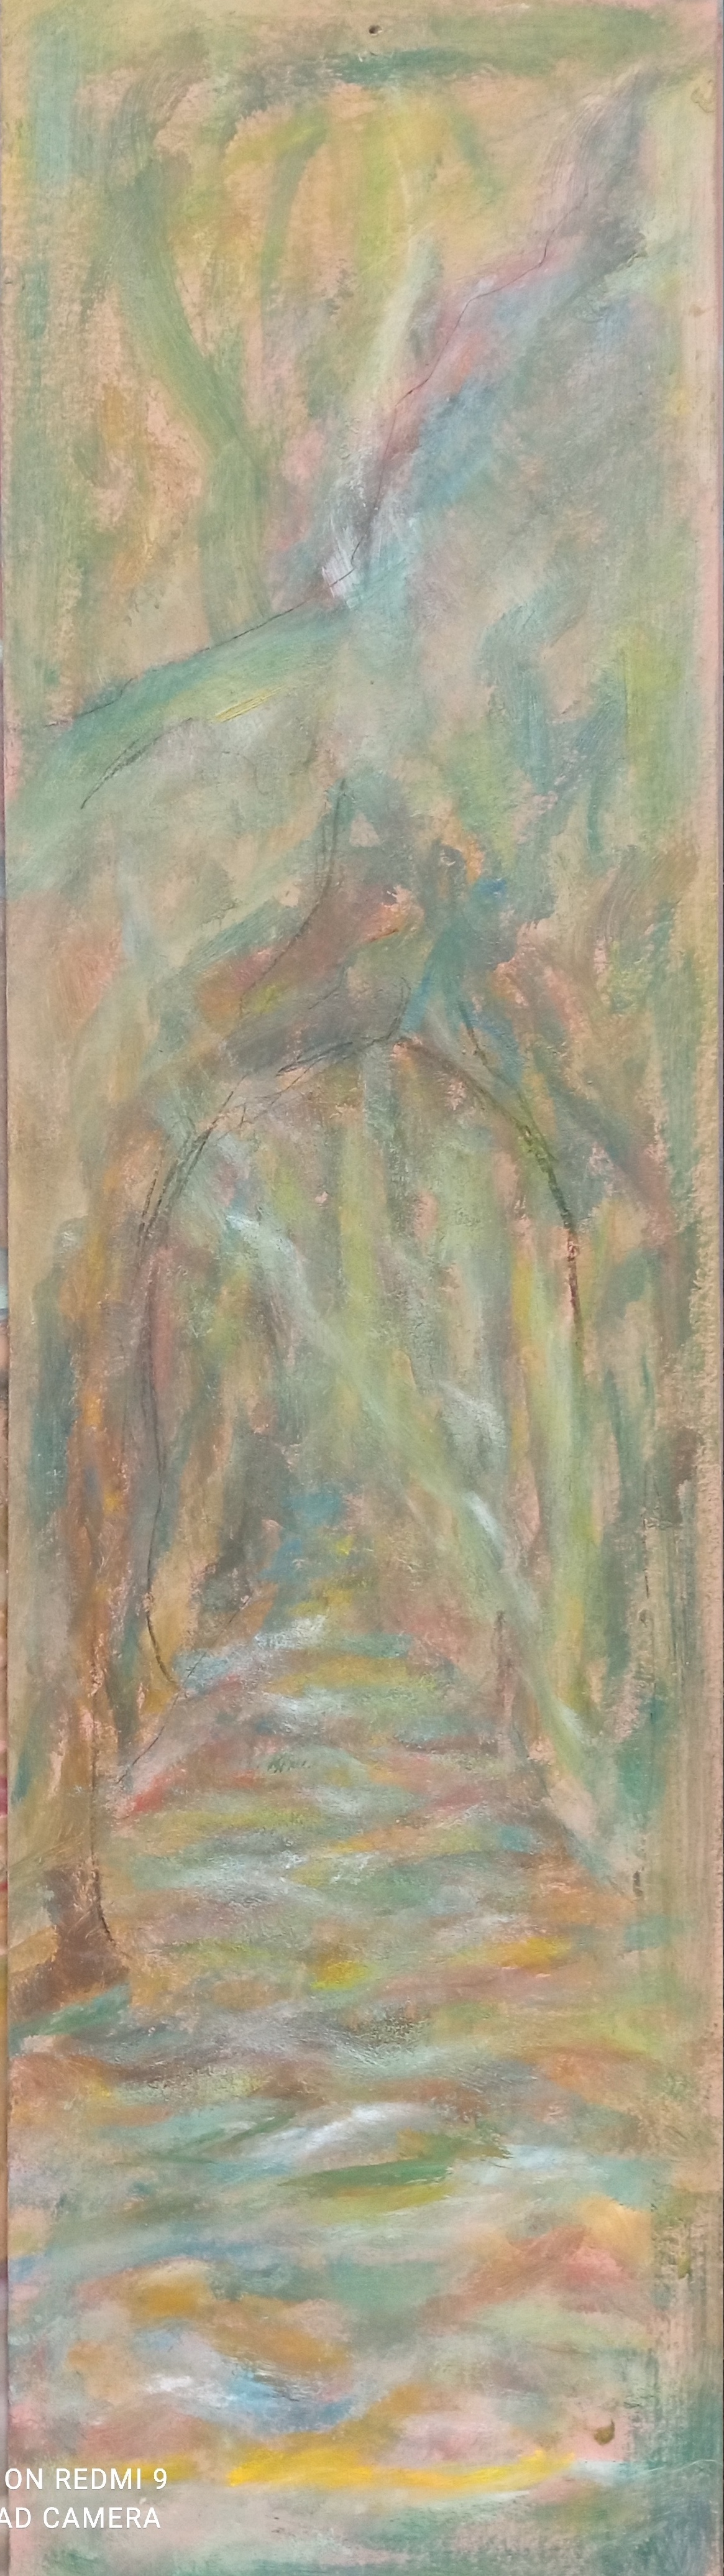
\includegraphics[width=\textwidth,height=\textheight,keepaspectratio]{assets/Tabla1.jpg}
    \newpage
    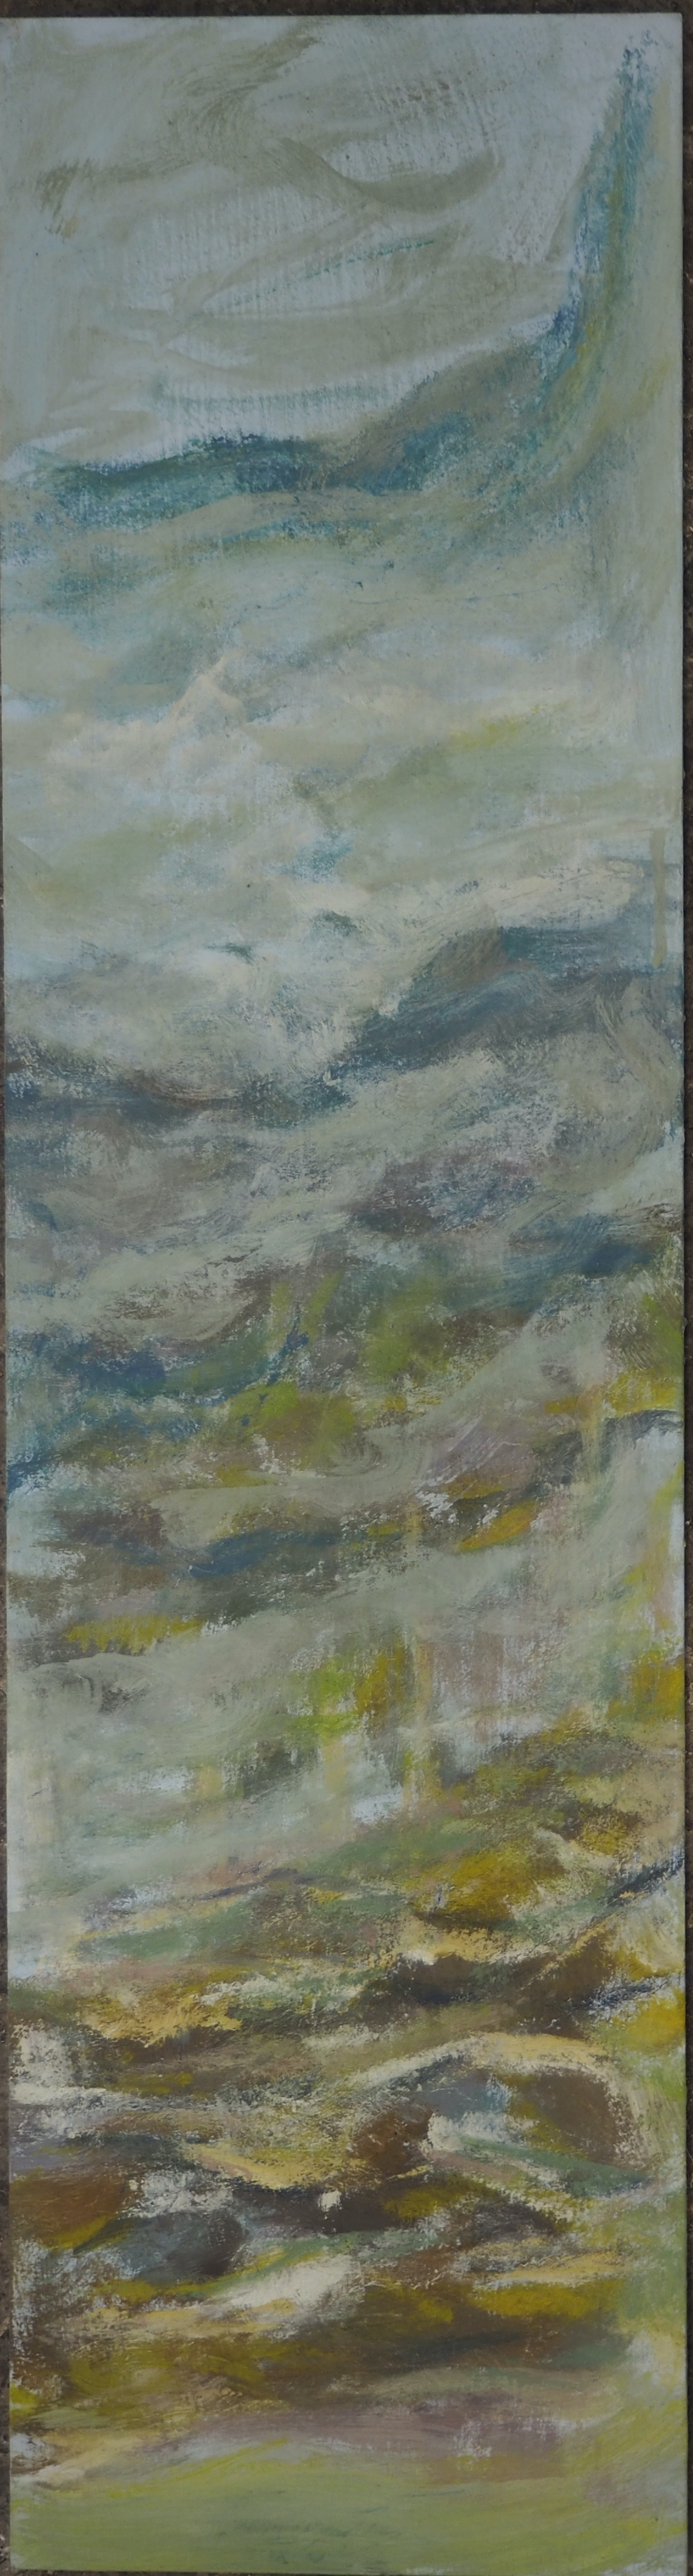
\includegraphics[width=\textwidth,height=\textheight,keepaspectratio]{assets/Tabla2.jpg}
    \newpage
    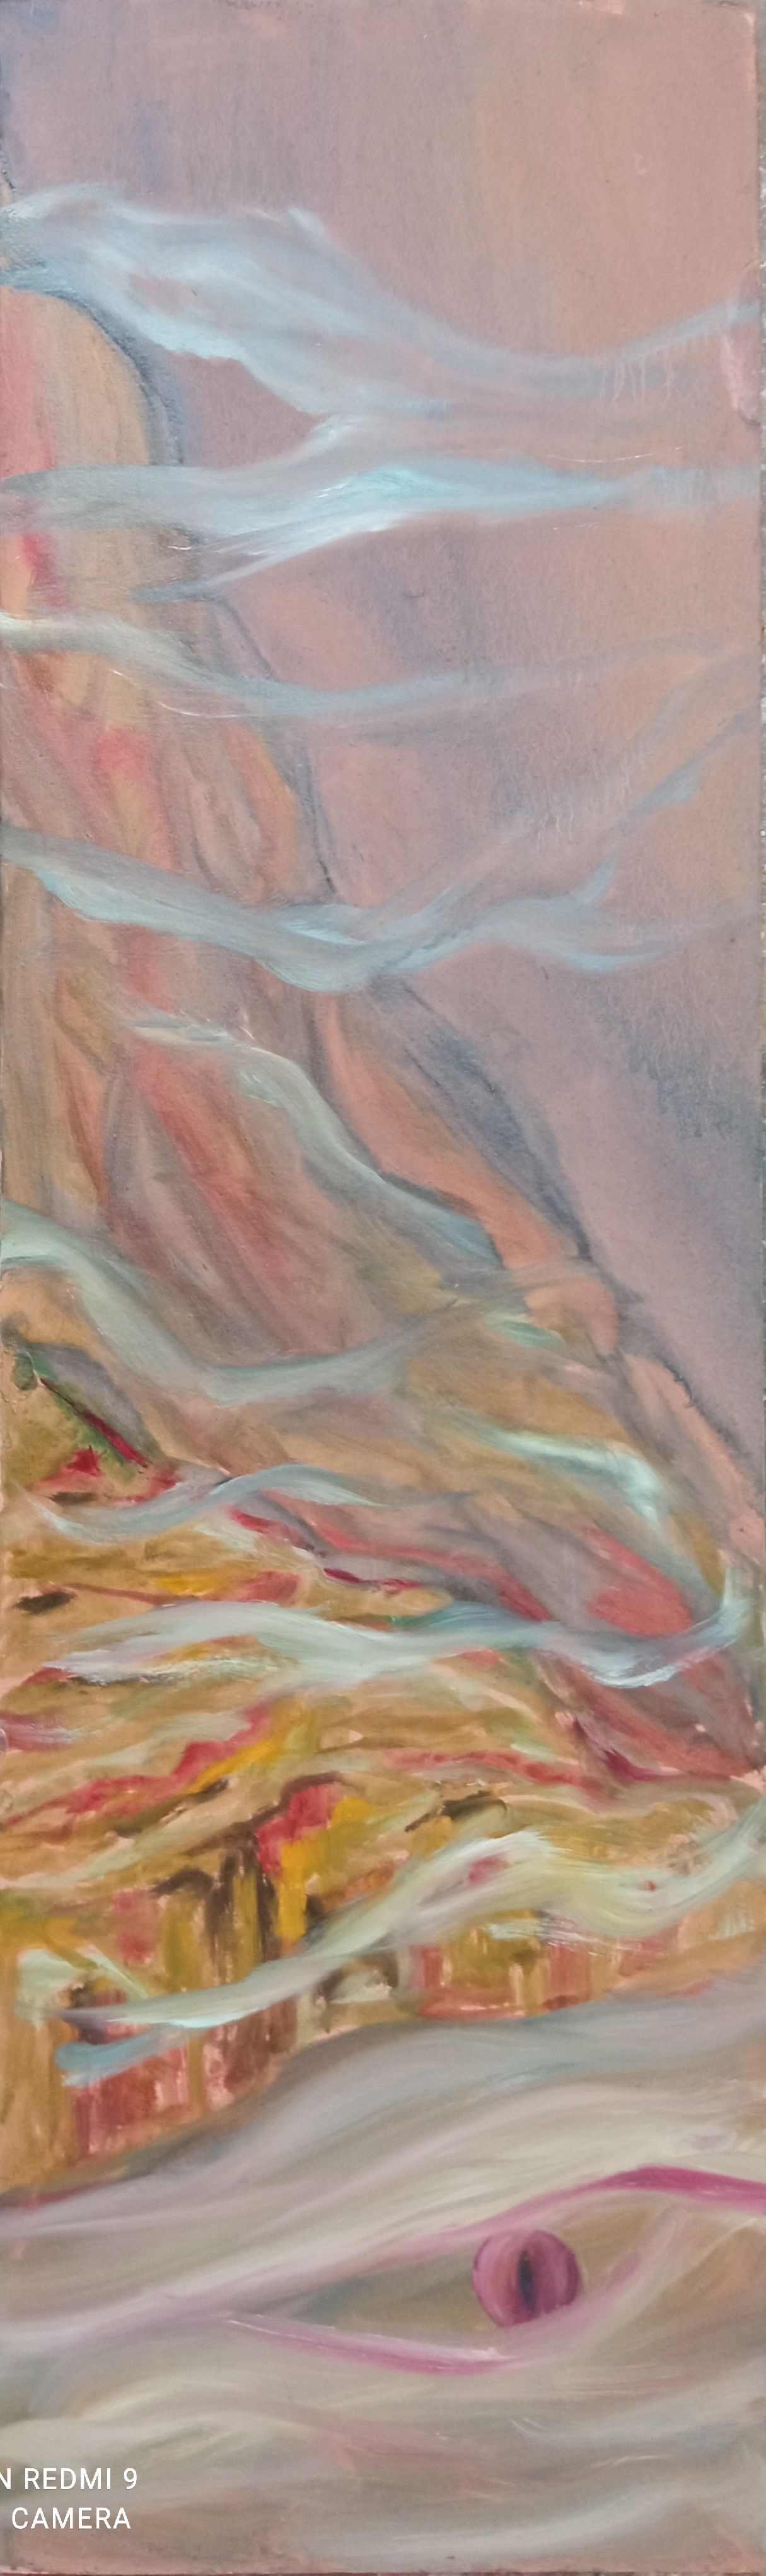
\includegraphics[width=\textwidth,height=\textheight,keepaspectratio]{assets/Tabla3.jpg}
    \newpage
    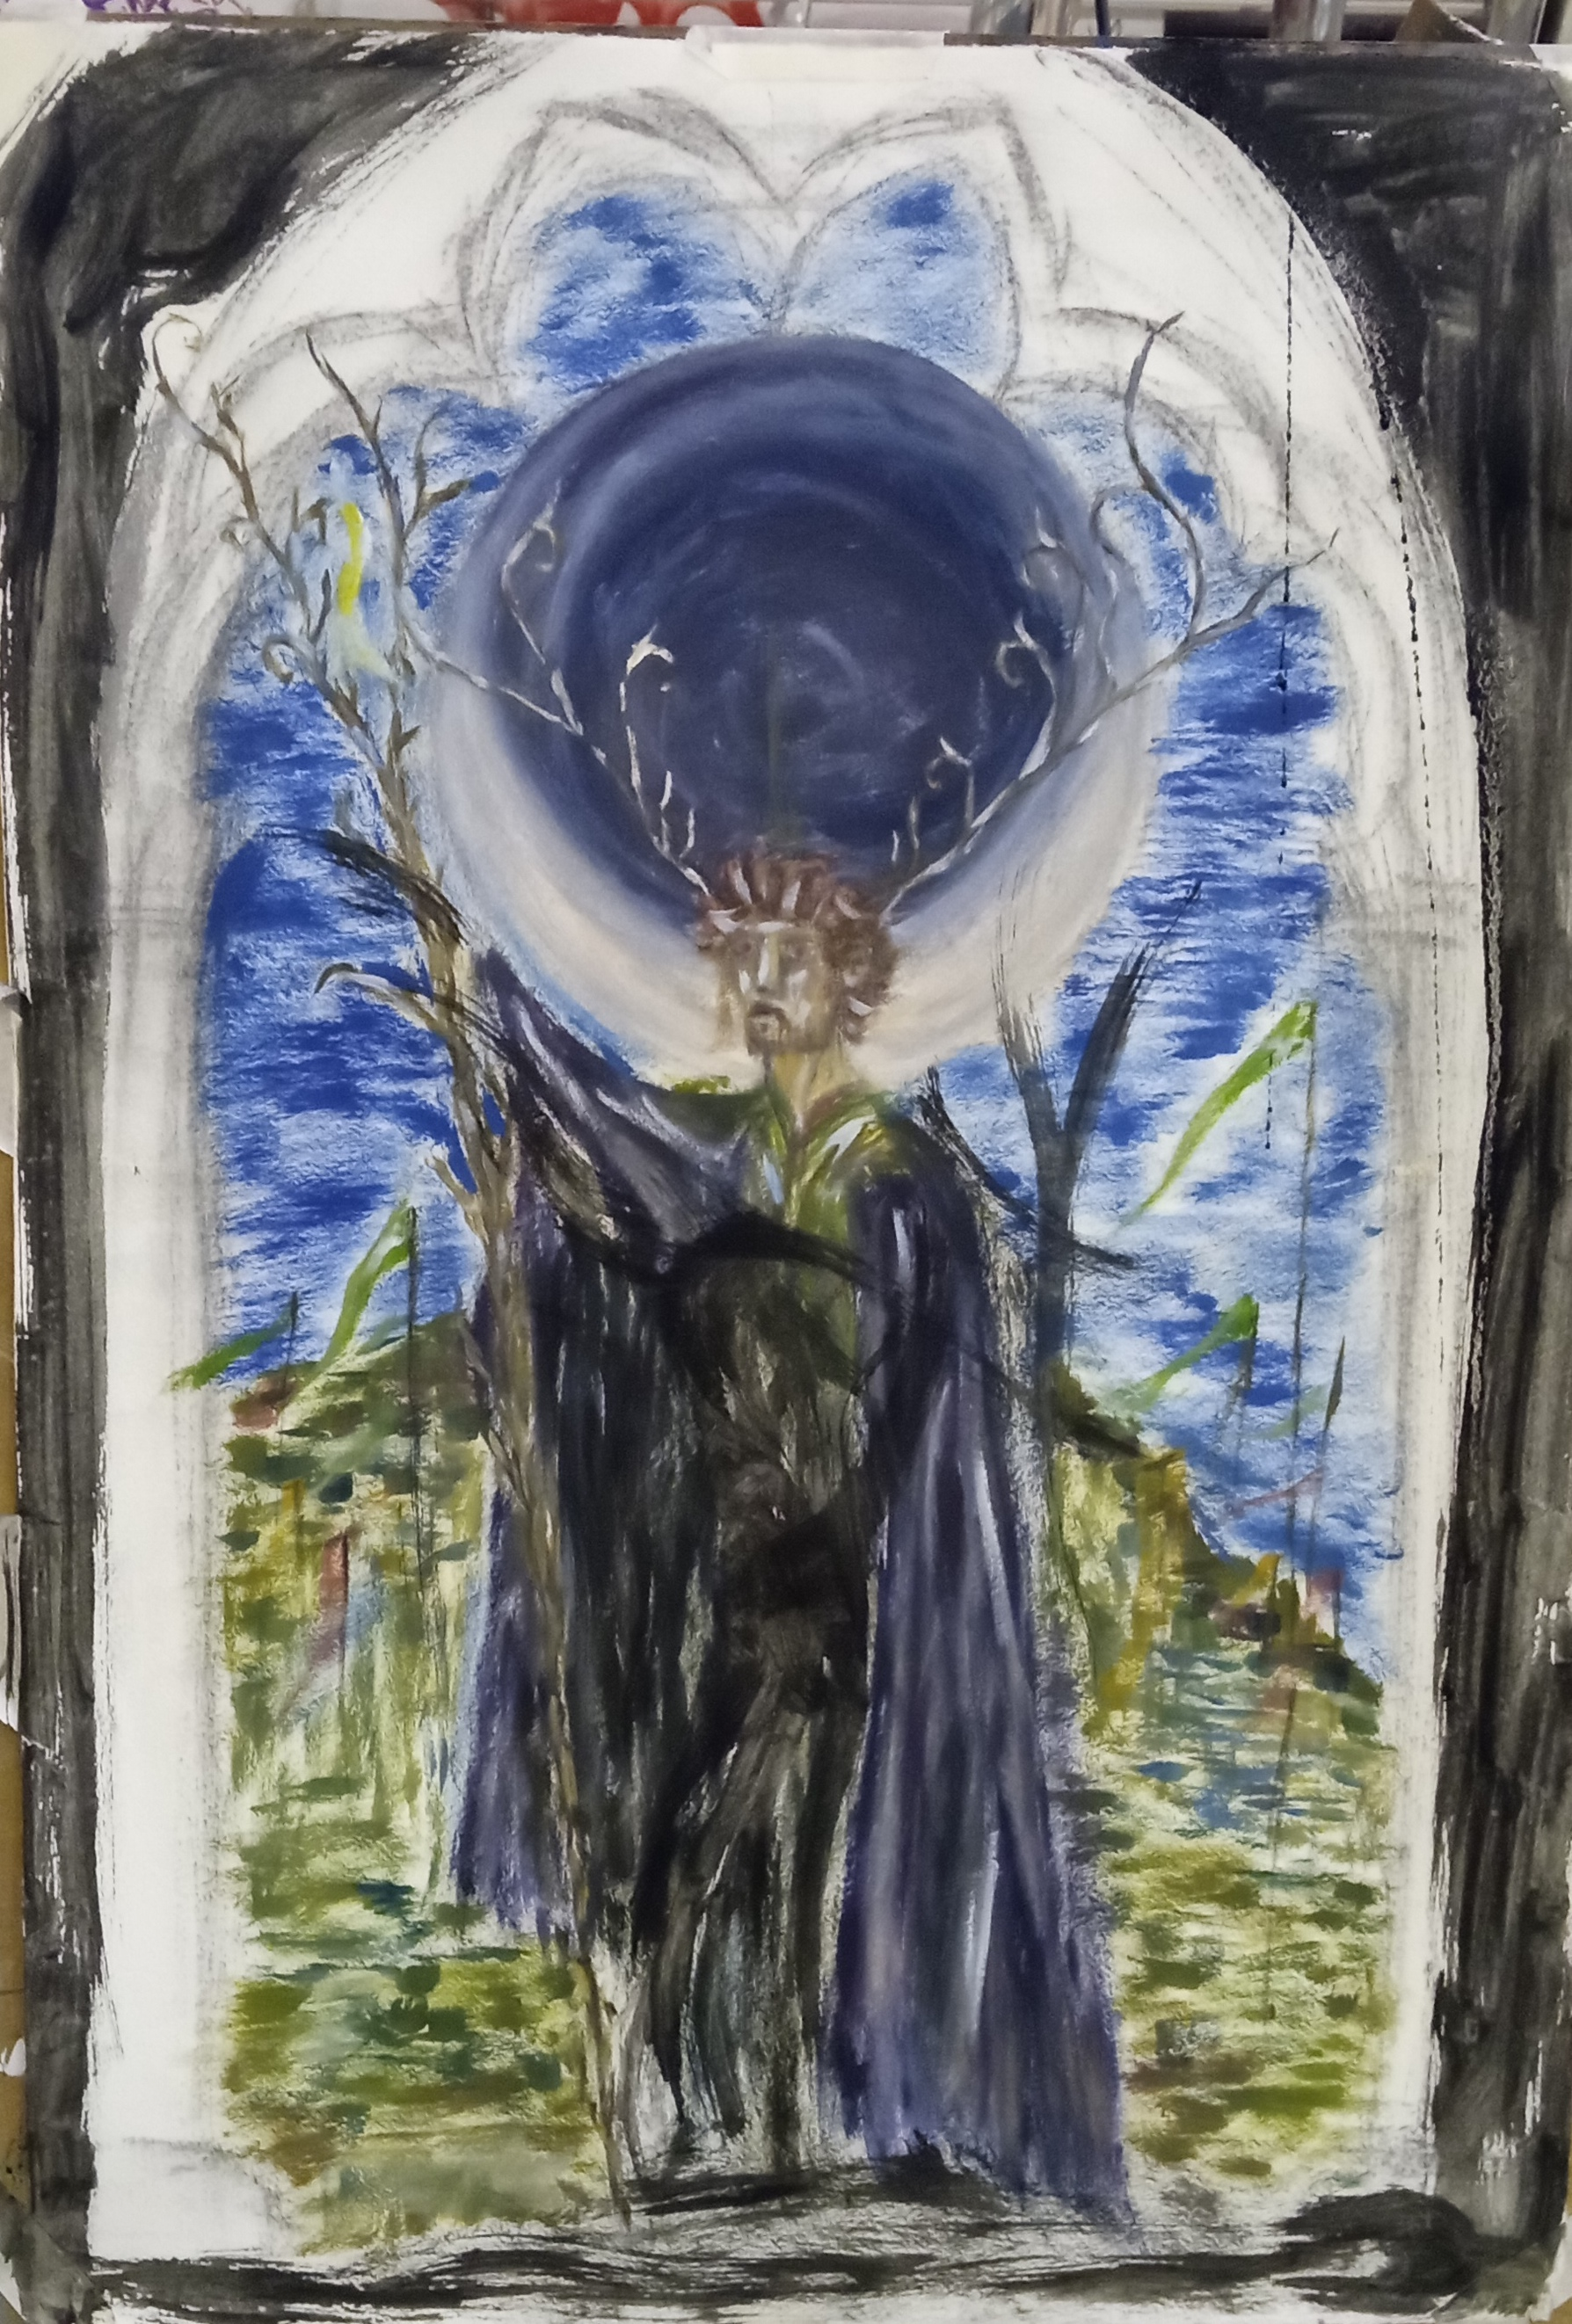
\includegraphics[width=\textwidth,height=\textheight,keepaspectratio]{assets/Final.jpg}
    \newpage
    \includegraphics[width=\textwidth,height=\textheight,keepaspectratio]{assets/torres.jpeg}
    \newpage
    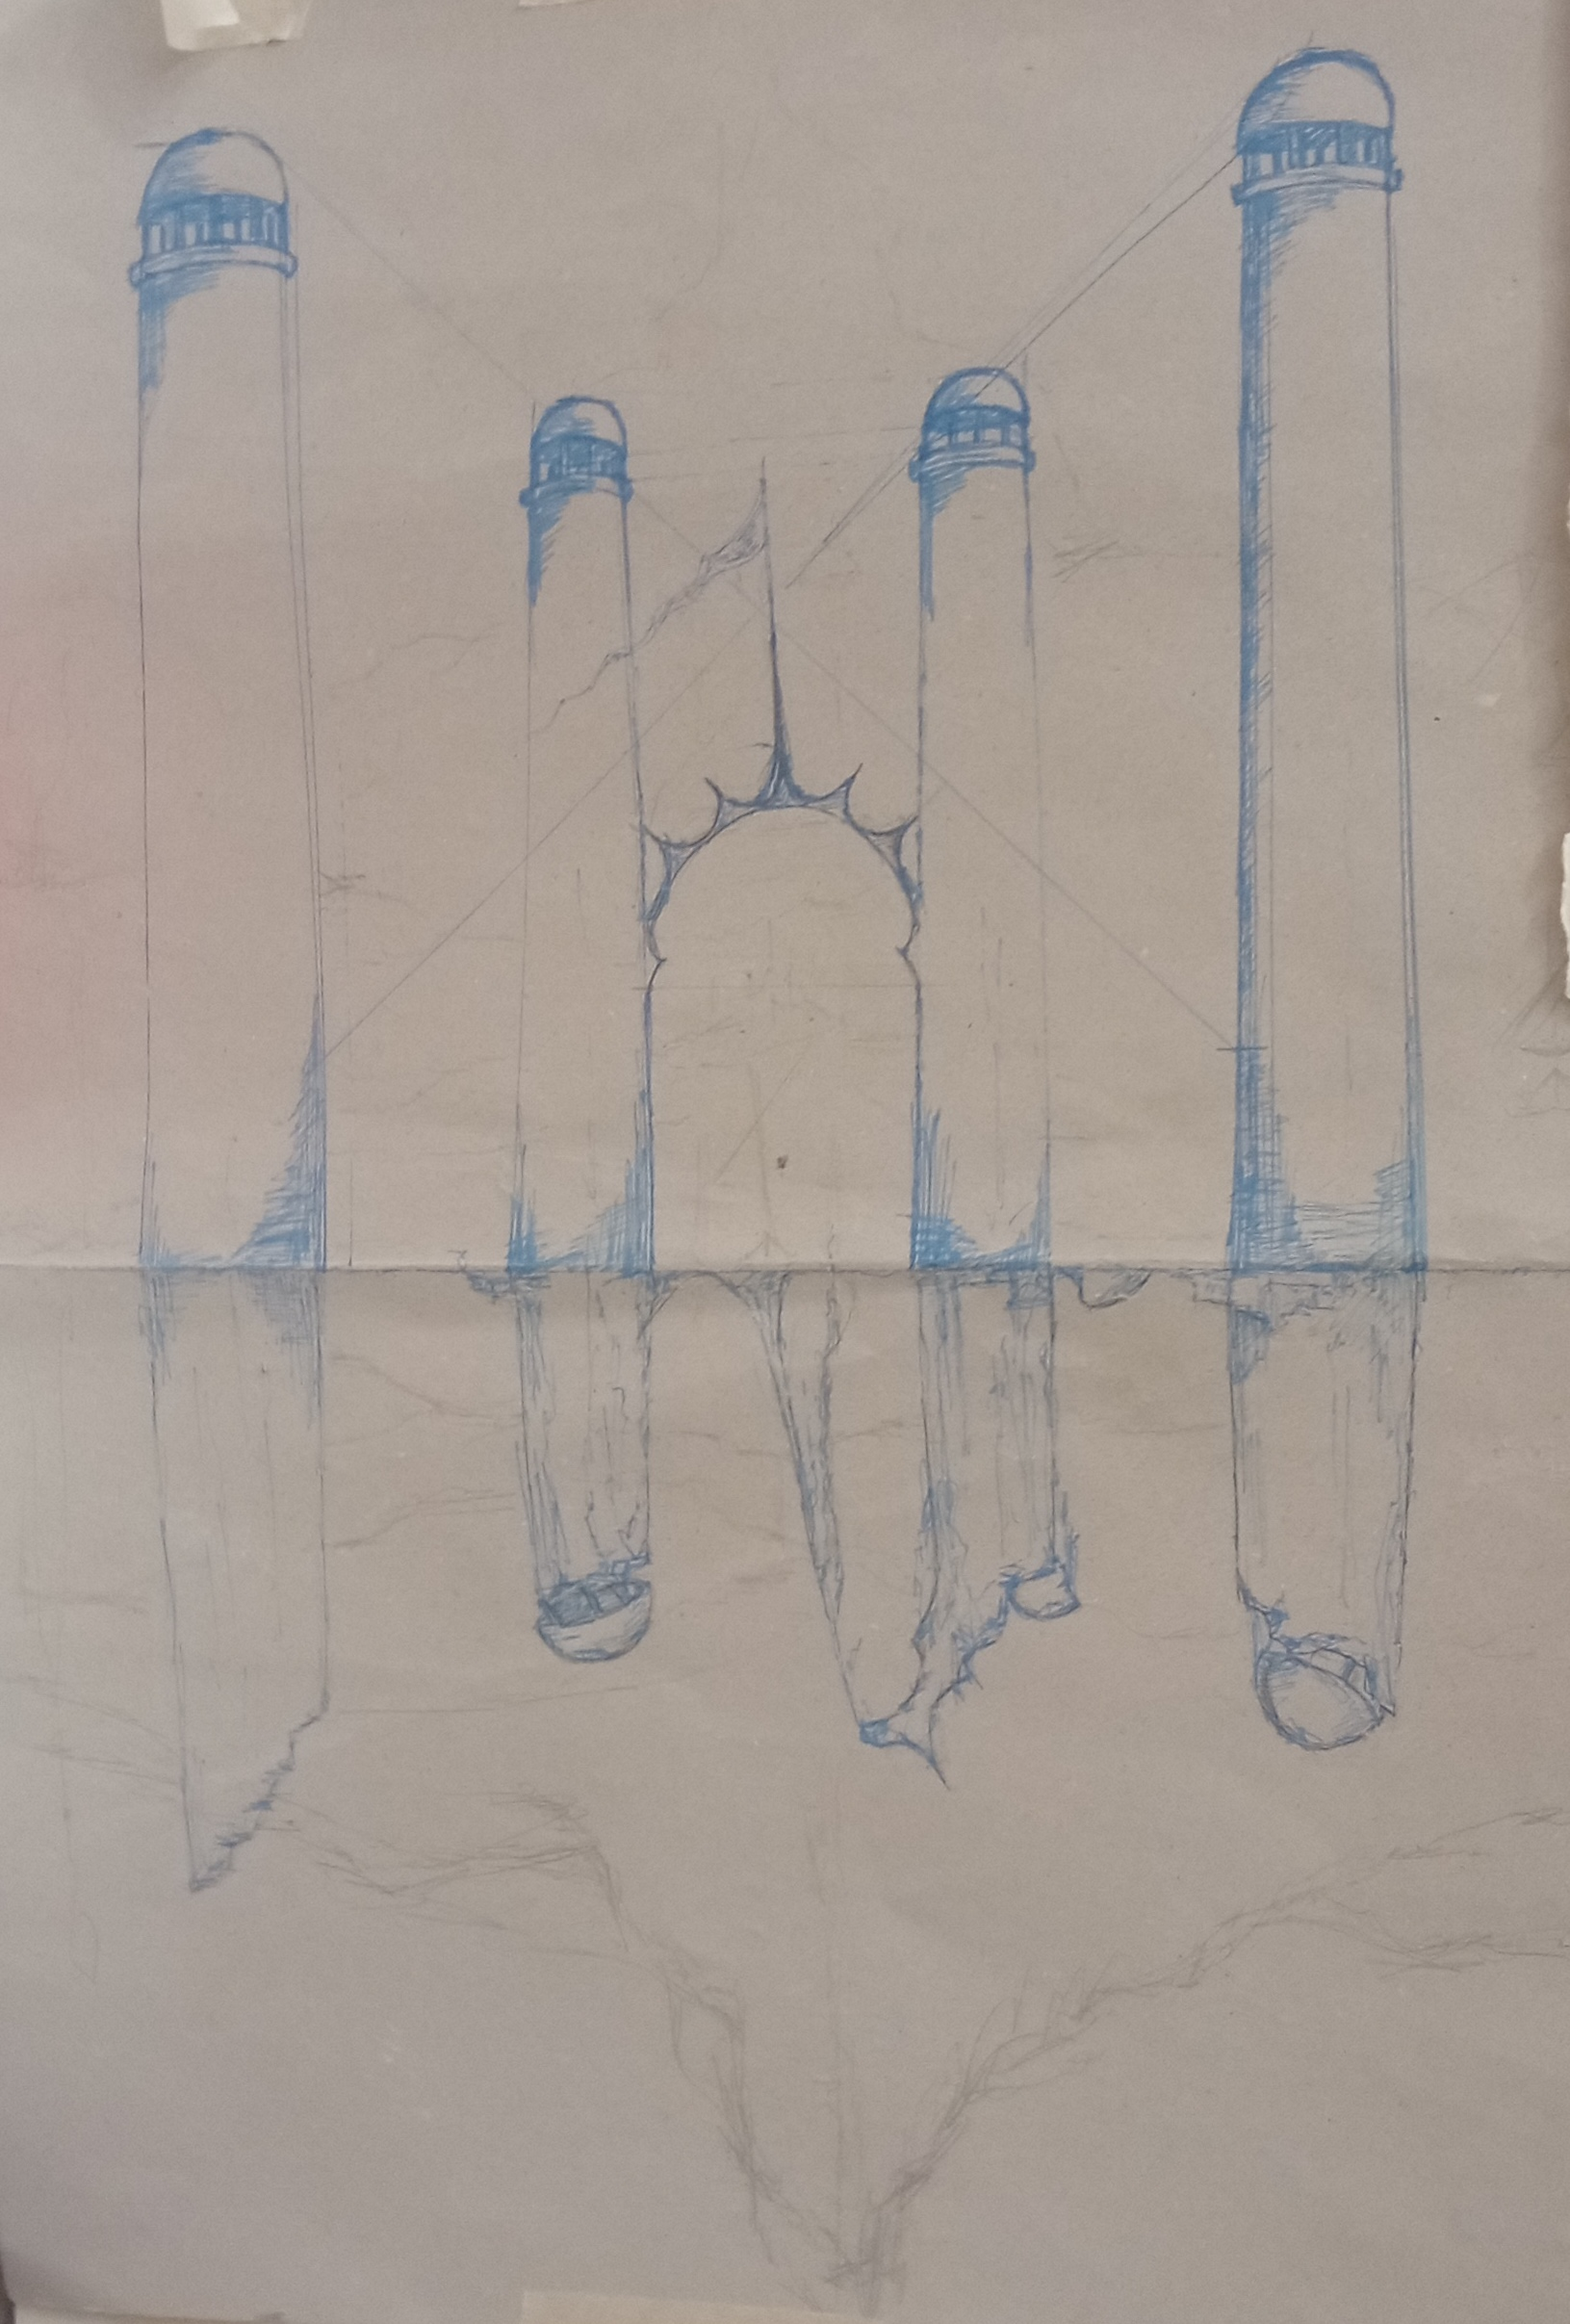
\includegraphics[width=\textwidth,height=\textheight,keepaspectratio]{assets/bocetorres.JPG}
    \newpage
    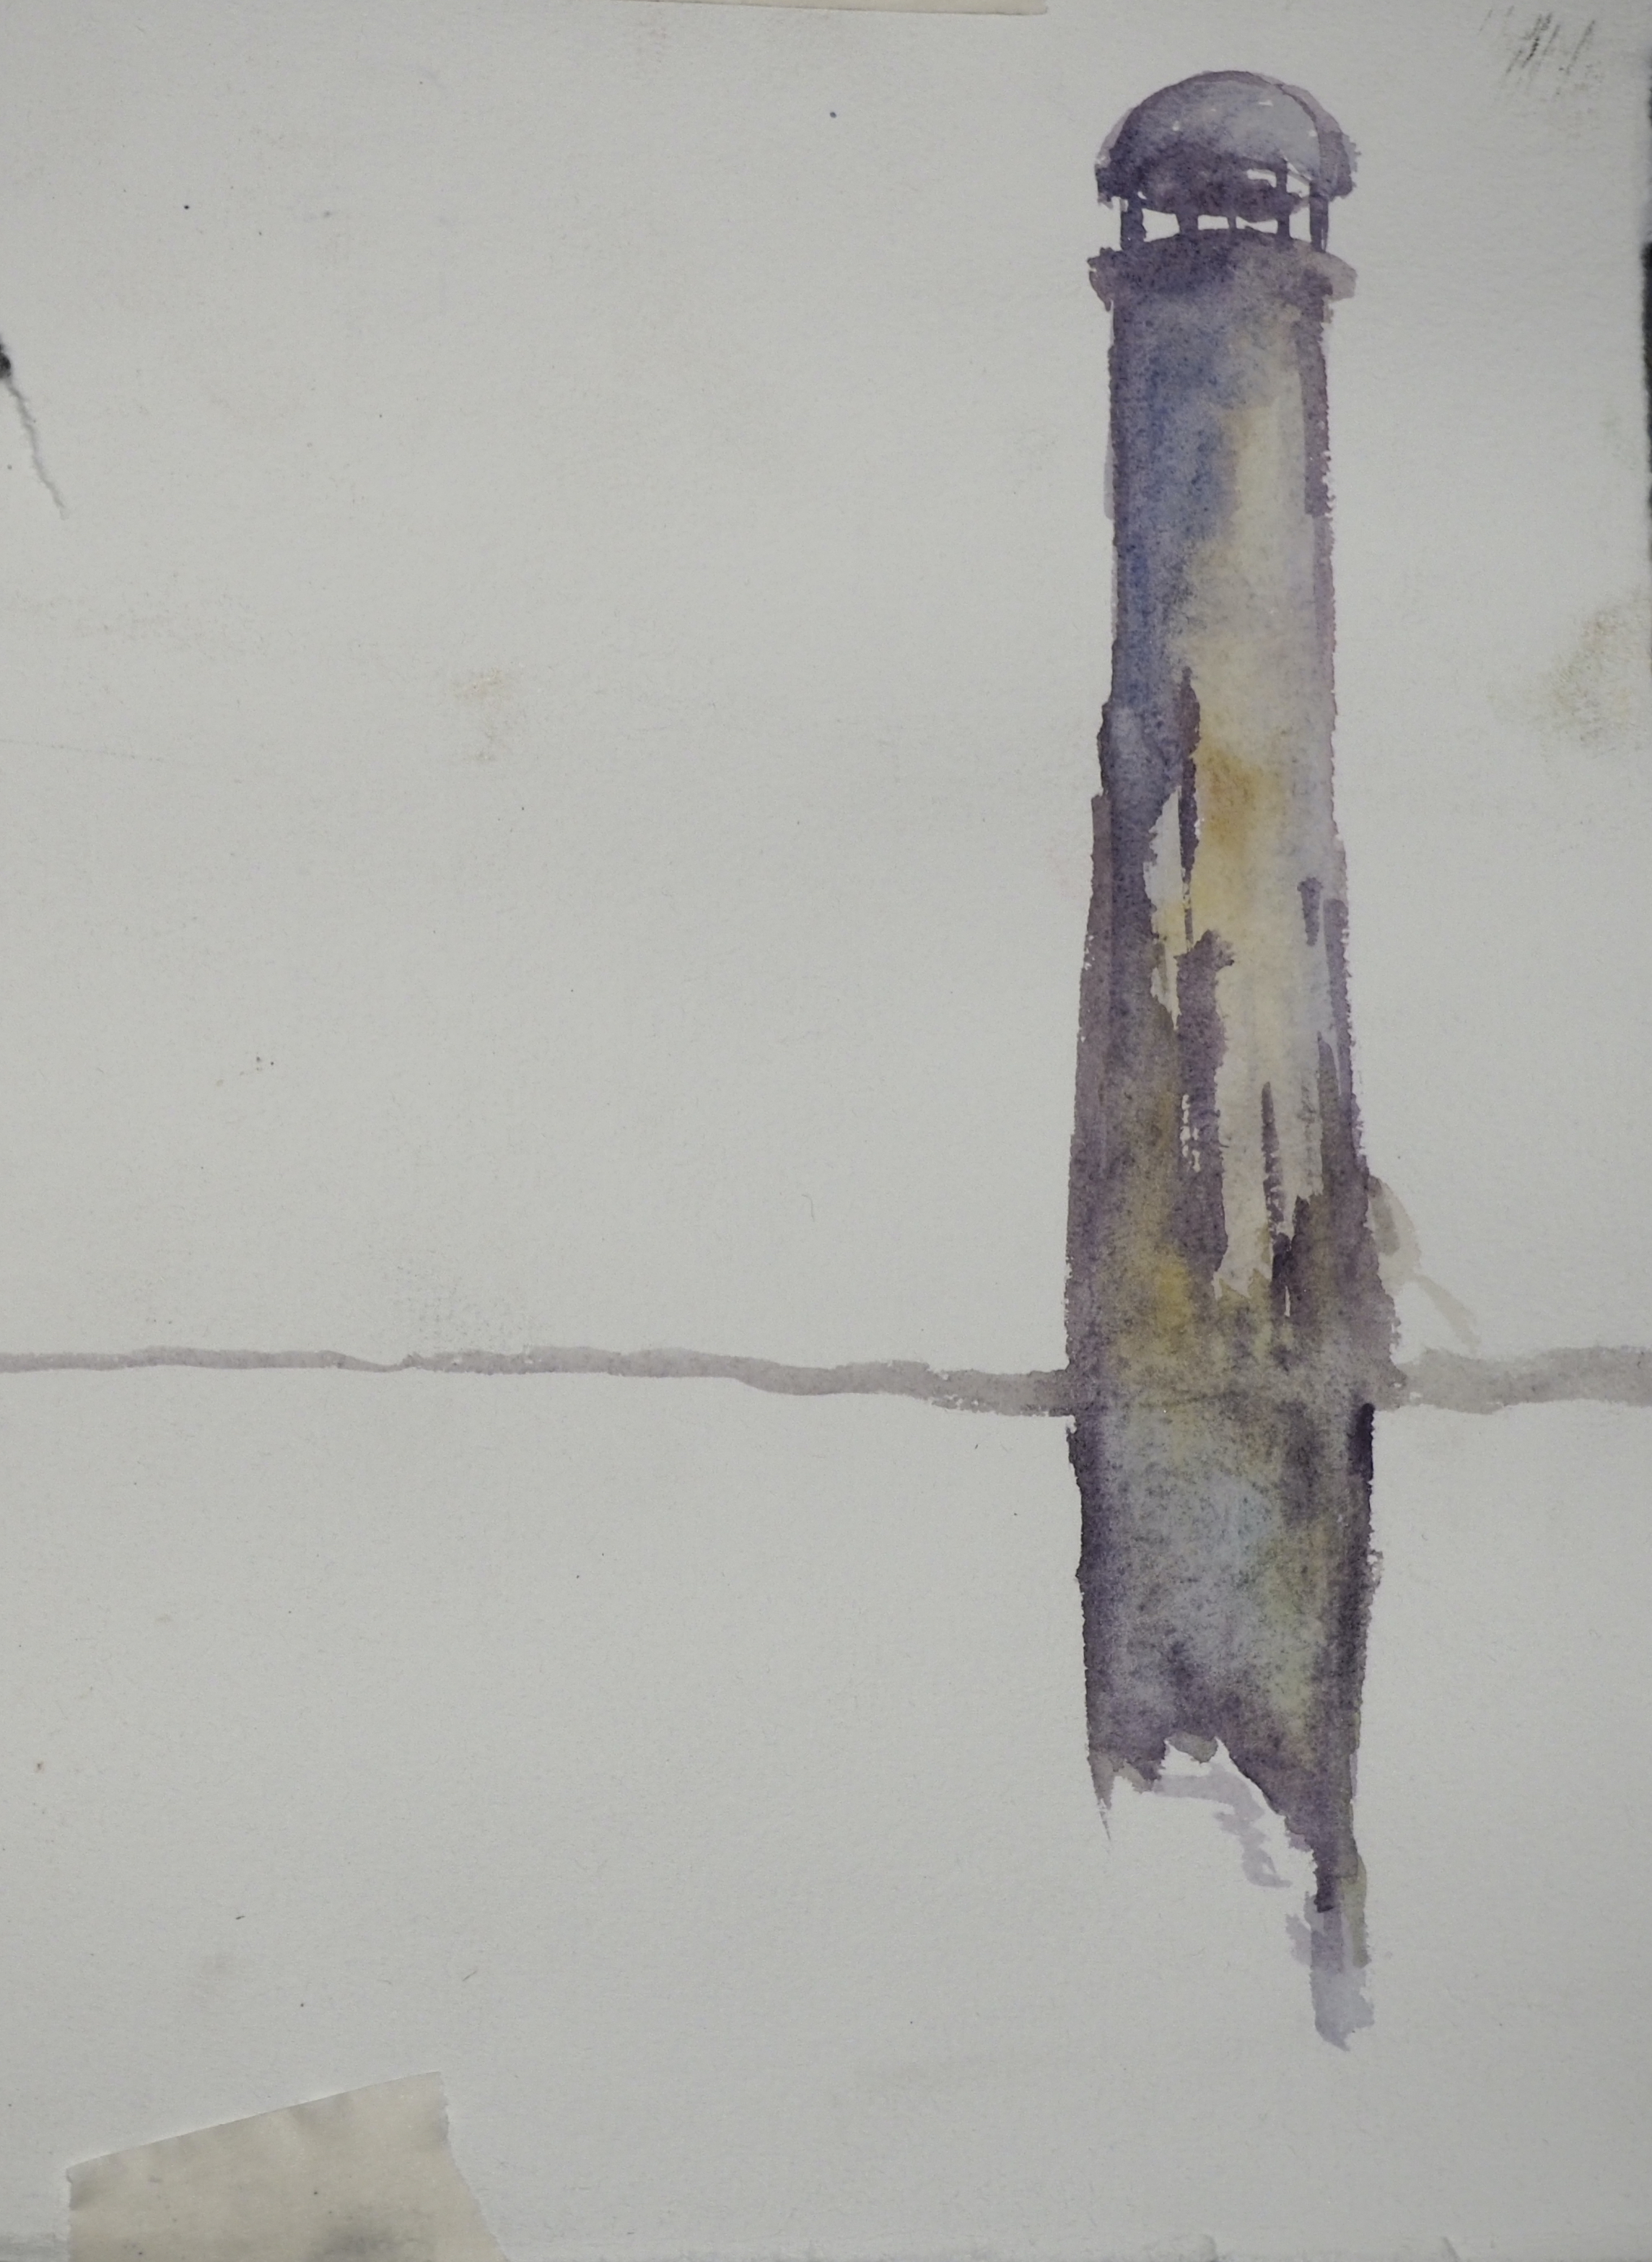
\includegraphics[width=\textwidth,height=\textheight,keepaspectratio]{assets/faro.JPG}
    \newpage
    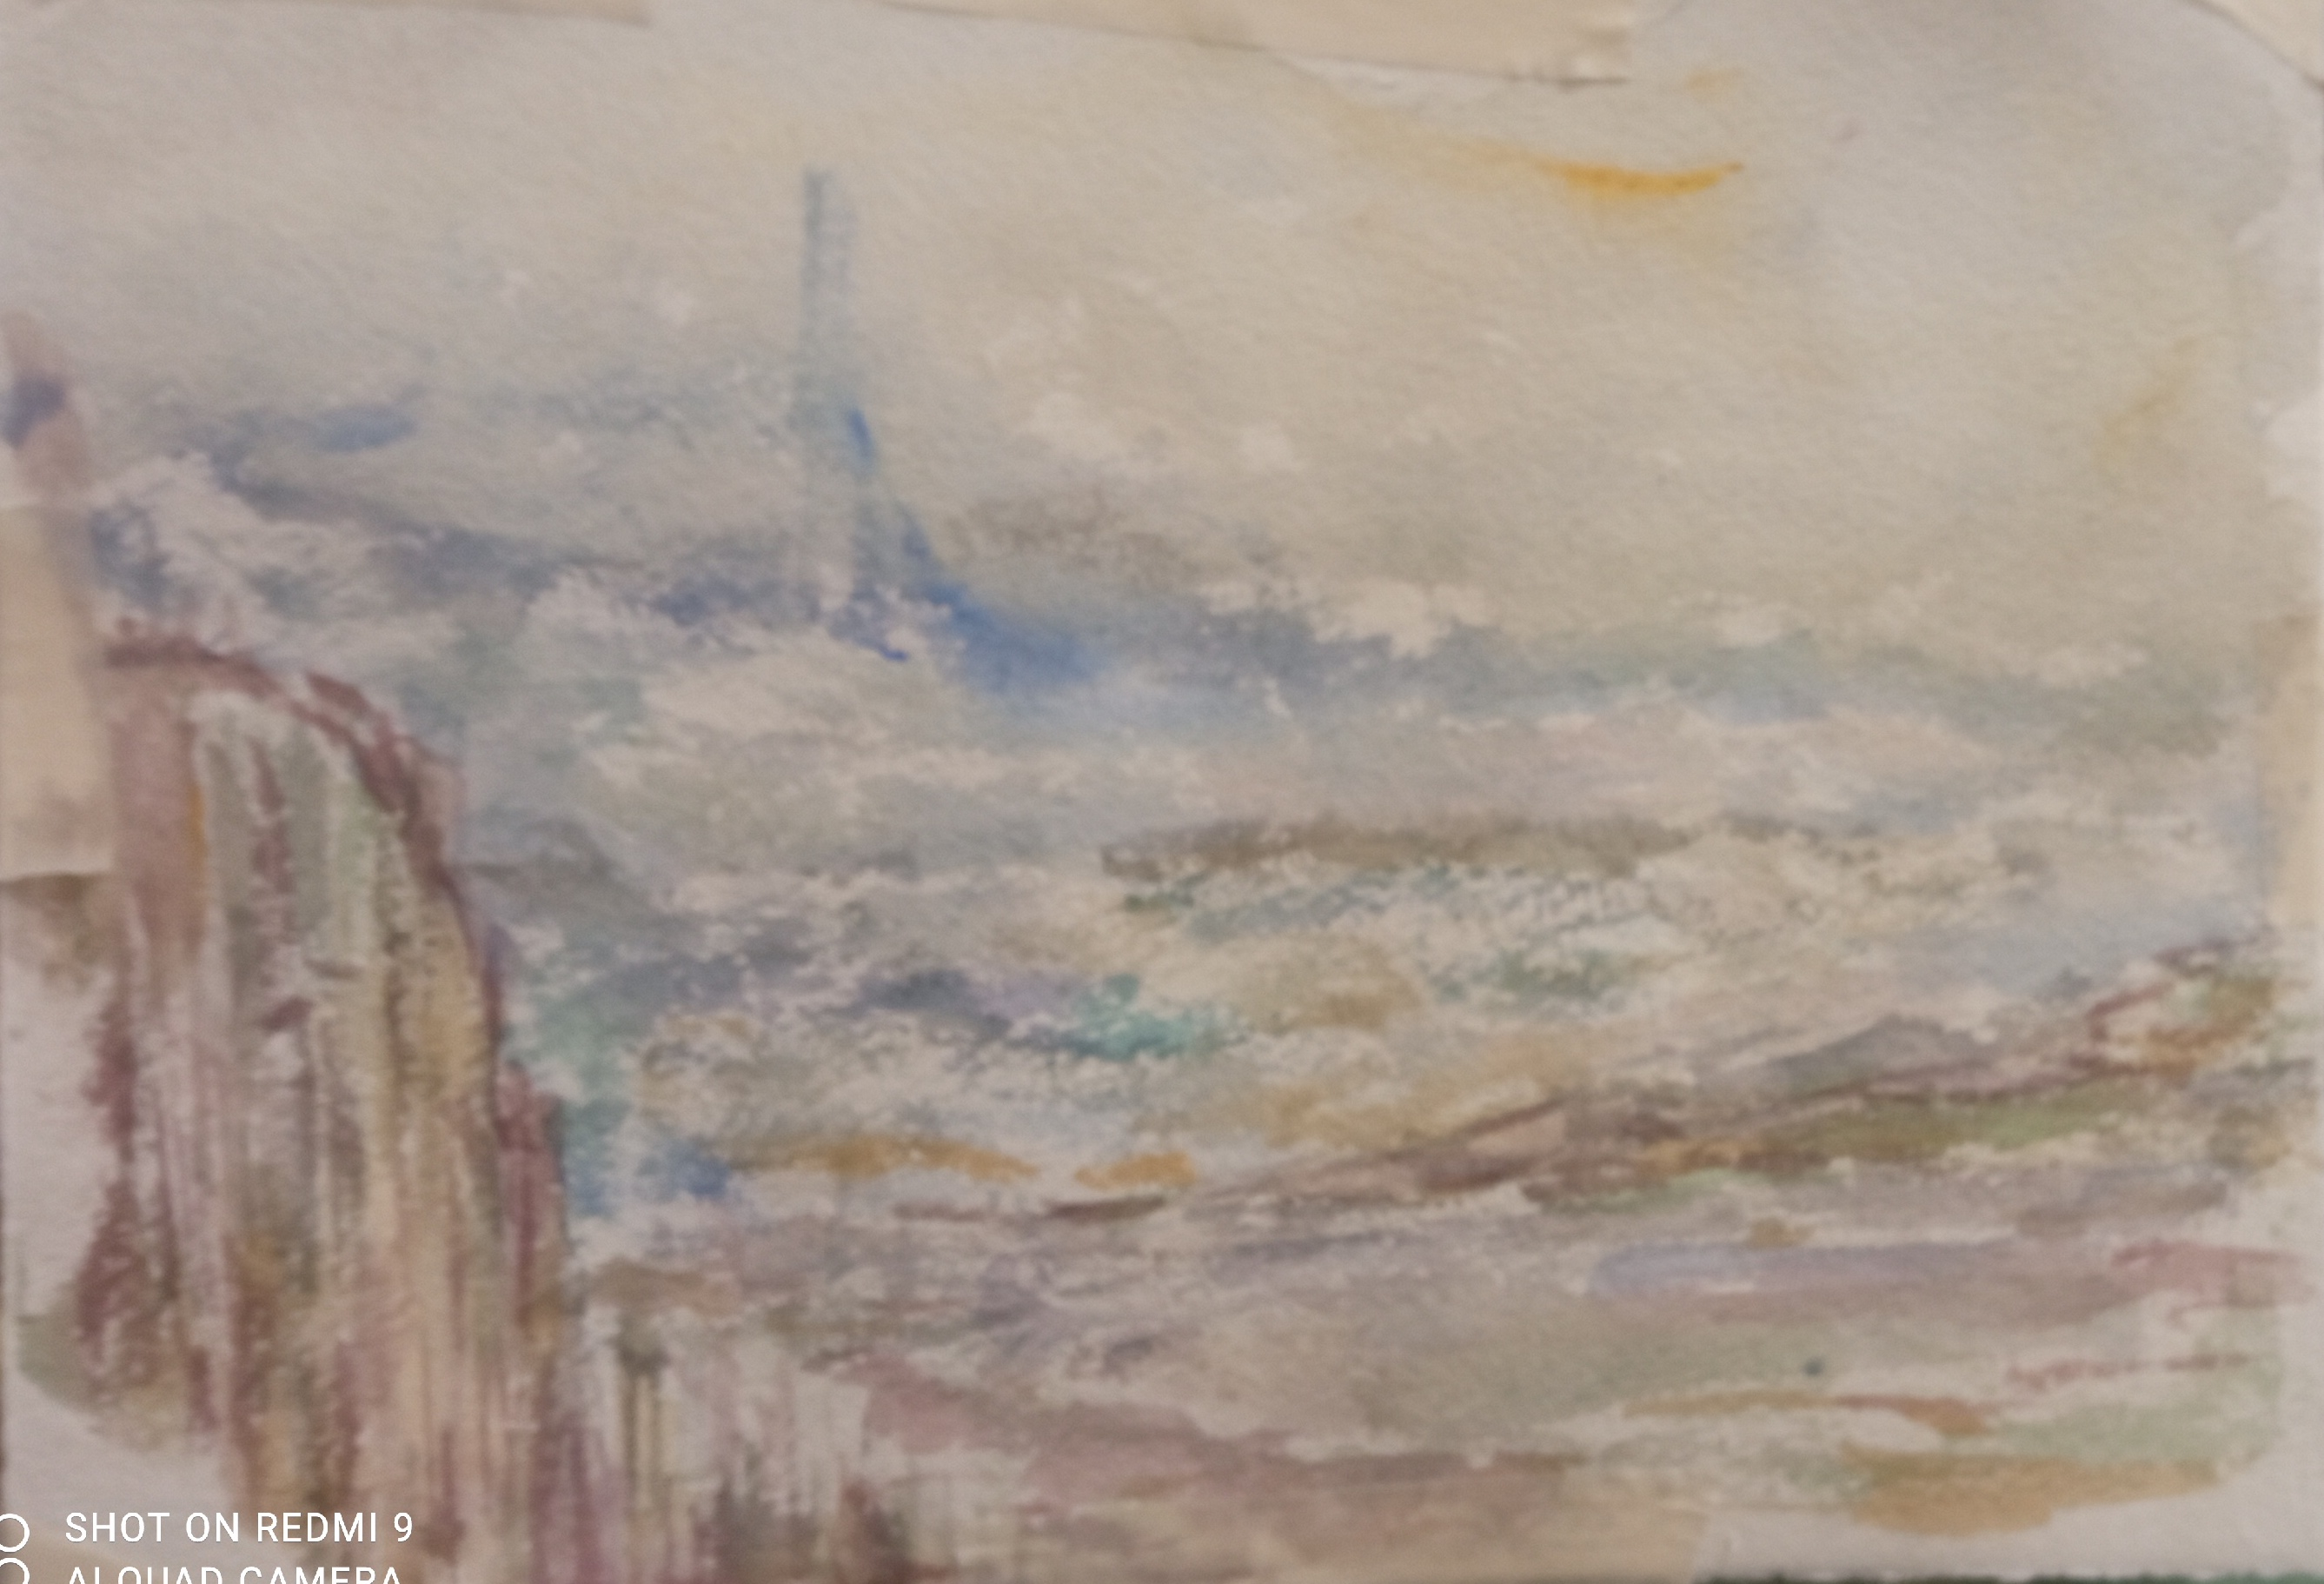
\includegraphics[width=\textwidth,height=\textheight,keepaspectratio]{assets/nubes.JPG}
    \newpage
    \includegraphics[width=\textwidth,height=\textheight,keepaspectratio]{assets/arbol.JPG}
    \newpage
    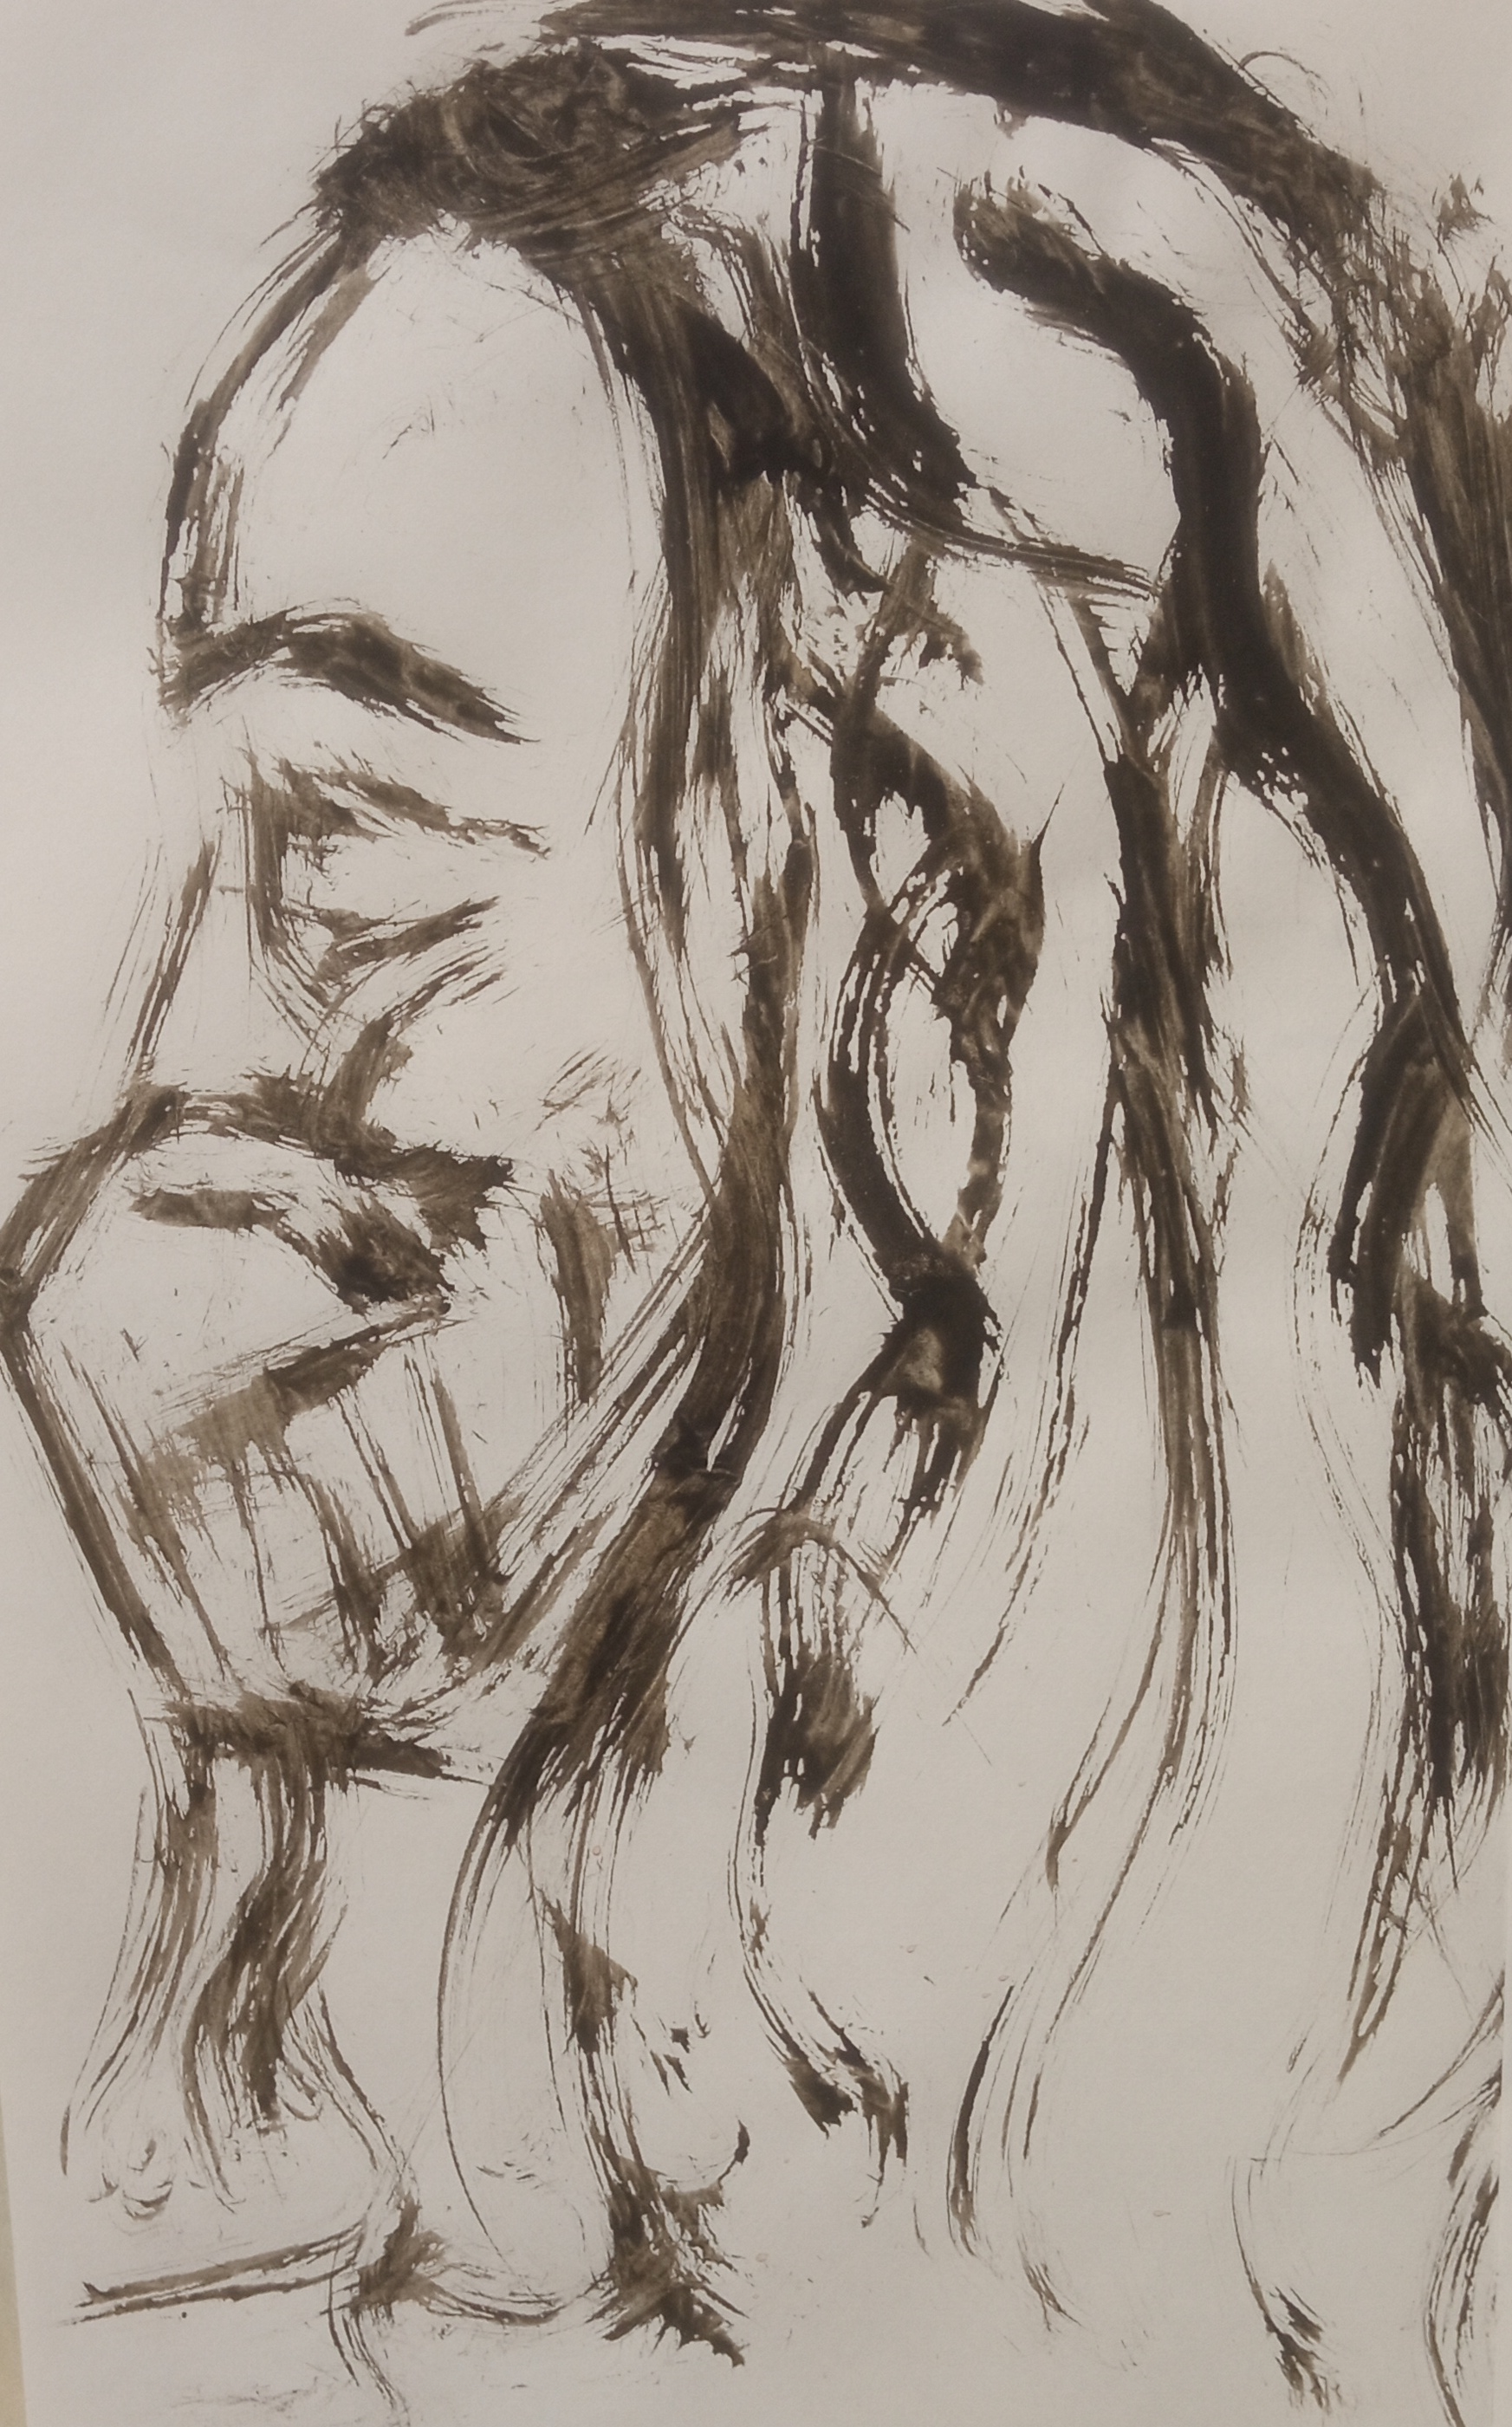
\includegraphics[width=\textwidth,height=\textheight,keepaspectratio]{assets/sofi.JPG}
    \newpage
  \end{center}
  \myemptypage{}
    
\newpage
\printendnotes{}
\newpage
\nocite{*}
\addcontentsline{toc}{chapter}{Referencias}
\printbibliography{}
\end{document}